\def\dbcol{double column single spacing}
\ifdefined\dbcol
\ifdefined\ACM
	\documentclass{sig-alternate-10pt}
	\makeatletter
	\def\@copyrightspace{\relax}
	\makeatother
\else
	\documentclass[conference,10pt,letterpaper]{IEEEtran}
	\IEEEoverridecommandlockouts
	\makeatletter
	\def\ps@headings{%
	\def\@oddhead{\mbox{}\scriptsize\rightmark \hfil \thepage}%
	\def\@evenhead{\scriptsize\thepage \hfil \leftmark\mbox{}}%
	\def\@oddfoot{}%
	\def\@evenfoot{}}
	\makeatother
\fi

\setlength{\fboxsep}{0pt}
\setlength{\fboxrule}{0pt}

\usepackage[left=.5in,right=.5in,top=.55in,bottom=.5in]{geometry}
\else
	\documentclass[conference,12pt,onecolumn]{IEEEtran}
\fi

\ifdefined\COMSOC%\ifCLASSOPTIONcompsoc
  \usepackage[nocompress]{cite}%1,2,3,4 will not be compressed as 1-4
\else
  \usepackage{cite} % normal IEEE
\fi
\ifdefined\ACM %ACM has Option clash for package graphicx
	\usepackage{amsmath}
\else
	\usepackage[cmex10]{amsmath} %ACM conflicts with cmex10 option
	\usepackage{amsthm} %ACM conflicts with this on \proof
%\ifCLASSINFOpdf
	\usepackage[pdftex]{graphicx} %\else \usepackage[dvips]{graphicx} \fi
\fi

\ifdefined\META     \usepackage{stmaryrd}    \fi %for \rrbracket

\newcommand{\begproof}{\ifdefined\dbcol\begin{IEEEproof}\else\begin{proof}\fi}
\newcommand{\Endproof}{\ifdefined\dbcol\end{IEEEproof}\else\end{proof}\fi}
\newcommand{\metacom}[1]{\ifdefined\META\bluepure{$\blacktriangleright$}#1\bluepure{$\rrbracket$}\fi}
\newcommand{\metafoot}[1]{\ifdefined\META\footnote{\bluepure{$\blacktriangleright$}#1}\fi}

%\usepackage{mdwmath}
%\usepackage{mdwtab}
% Also highly recommended is Mark Wooding's extremely powerful MDW tools,
% especially mdwmath.sty and mdwtab.sty which are used to format equations
% and tables, respectively. The MDWtools set is already installed on most
% LaTeX systems.

\usepackage[font=small]{subfig} %font=scriptsize/small/footnotesize
%--------- INFOCOM'14 camera-ready version used below -----------
%\usepackage[caption=false,textfont=sf,font=footnotesize]{subfig}
%\usepackage[font=small]{caption}%footnotesize
	%Package caption Warning: Unsupported document class (or package) detected, (caption)  usage of the caption package is not recommended.
%--------- INFOCOM'14 camera-ready version used above -----------

\usepackage{hyperref} %for special characters and smart line breaking in URL

%%%%%%%%%%%%% MY OWN ADDED PACKAGES %%%%%%%%%%%%%%%%%

\usepackage{amssymb}
\usepackage{bbm} %\mathbbm 1 %\newcommand{\ind}{1\hspace{-2.3mm}{1}}
\usepackage{verbatim}
\usepackage{color}
\usepackage[normalem]{ulem}%{soul}
%\usepackage{algorithmic}
%\usepackage{algorithm}
\usepackage[ruled,lined,linesnumbered]{algorithm2e}
%\usepackage{parskip}
%\usepackage{fullpage} %1-inch margin
%\usepackage[margin=1.5cm]{geometry}
%\usepackage[left=1.5cm,right=1.5cm,top=2cm,bottom=2cm,nohead]{geometry}%,nofoot
%\usepackage{anysize}
%\marginsize{2cm}{2cm}{1cm}{1cm} %\marginsize{left}{right}{top}{bottom}
%%%%%%%%%%%%%%%%%%%%%%%%%%%%%%%%%

% fontsize illustration: http://tex.stackexchange.com/questions/24599/what-point-pt-font-size-are-large-etc
%Command             10pt    11pt    12pt
%\tiny               5       6       6
%\scriptsize         7       8       8
%\footnotesize       8       9       10
%\small              9       10      10.95
%\normalsize         10      10.95   12
%\large              12      12      14.4
%\Large              14.4    14.4    17.28
%\LARGE              17.28   17.28   20.74
%\huge               20.74   20.74   24.88
%\Huge               24.88   24.88   24.88

\newtheorem{thm}{Theorem}
\newtheorem{lem}{Lemma}
\newtheorem{prop}{Proposition}
\newtheorem{coro}{Corollary}
\newtheorem{defn}{Definition}
\newtheorem{hypo}{Hypothesis}
\newtheorem{conj}{Conjecture}
\newtheorem{ex}{Example}
\newcommand{\eref}[1]{Eq.~\eqref{#1}} %IEEE style manual suggests using (1) only
\newcommand{\fref}[1]{Fig.~\ref{#1}}
\newcommand{\tref}[1]{Table~\ref{#1}}
\newcommand{\sref}[1]{Section~\ref{#1}}
\newcommand{\thmref}[1]{Theorem~\ref{#1}}
\newcommand{\lref}[1]{Lemma~\ref{#1}}
\newcommand{\pref}[1]{Proposition~\ref{#1}}
\newcommand{\cref}[1]{Corollary~\ref{#1}}
\newcommand{\dref}[1]{Definition~\ref{#1}}
%\newcommand{\href}[1]{Hypothesis~\ref{#1}}
\newcommand{\jref}[1]{Conjecture~\ref{#1}}
\newcommand{\aref}[1]{Algorithm~\ref{#1}}
\newcommand{\pcref}[1]{Procedure~\ref{#1}}
\newcommand{\vect}[1]{\boldsymbol{#1}}
\newcommand{\veclong}[1]{\overrightarrow{#1}} %but the arrow is a bit too big
\newcommand{\sumiN}{\sum_{i=1}^N}
\newcommand{\sumin}{\sum_{i=1}^n}
\newcommand{\suml}{\sum_{l=1}^N}
\newcommand{\sumk}{\sum_{k=1}^N}
\newcommand{\prodi}{\prod_{i=1}^N}
\newcommand{\blue}[1]{{\color{blue}\dotuline{#1}}}
\newcommand{\bluepure}[1]{{\color{blue}{#1}}}
%\newcommand{\blue}[1]{#1}
\newcommand{\red}[1]{{\color{red}\dashuline{#1}}}
%\newcommand{\red}[1]{#1}
\newcommand{\tts}[1]{\tt\small{#1}}
\newcommand{\ttscr}[1]{\tt\scriptsize{#1}}
\newcommand{\ttfoot}[1]{\tt\footnotesize{#1}}
\newcommand{\its}[1]{\it\small{#1}}
\newcommand{\itscr}[1]{\it\scriptsize{#1}}
\newcommand{\itfoot}[1]{\it\footnotesize{#1}}
\newcommand{\eqv}{\Leftrightarrow}%\iff is quite long
\newcommand{\means}{\Rightarrow}
\newcommand{\eps}{\epsilon}
\newcommand{\ovl}{\overline}
\newcommand{\nn}{\nonumber}
\newcommand{\opd}{\operatorname{d}\!}
\renewcommand{\d}[2]{\frac{\opd#1}{\opd#2}} % for derivatives
\newcommand{\dd}[2]{\frac{\opd^2\!#1}{\opd#2^2}} % for double derivatives
\newcommand{\pd}[2]{\frac{\partial #1}{\partial #2}} % for partial derivatives
\newcommand{\pdd}[2]{\frac{\partial^2 #1}{\partial {#2}^2}} % for double partial derivatives
\newcommand{\pddd}[3]{\frac{\partial^2 #1}{\partial {#2} \partial {#3}}}
\newcommand{\inv}[1]{\frac{1}{#1}} %inverse
\DeclareMathOperator*{\argmax}{arg\,max}
\DeclareMathOperator*{\argmin}{arg\,min}
\DeclareMathOperator\erf{erf}
\DeclareMathOperator*{\E}{\mathbb{E}}% Expectation symbol; Using the starred version of \DeclareMathOperator makes sure subscripts goes _beneath_ the symbol in display mode.

%\floatname{algorithm}{Procedure}
%\renewcommand{\algorithmicrequire}{\textbf{Input:}}
%\renewcommand{\algorithmicensure}{\textbf{Output:}}

\hyphenation{op-tical net-works semi-conduc-tor}

\let\labelindent\relax
\usepackage{enumitem}

\def\figurename{Figure}\def\tablename{Table}

\usepackage{caption}
\captionsetup[table]{format=plain,labelformat=simple}


\usepackage{fancyhdr}
%\pagestyle{fancy} %commenting out this removes lines on other pages
\fancypagestyle{empty}{
  \fancyhf{}% Clear header/footer
  \fancyhead[C]{\footnotesize{T. Luo, S. S. Kanhere, H-P. Tan, F. Wu, and H. Wu, ``Crowdsourcing with Tullock contests: A new perspective'', {\it Proc. IEEE INFOCOM}, 2015, pp. 2515-2523.}}
}

\usepackage{datetime}
\title{Crowdsourcing with Tullock Contests:\\A New Perspective}
\author{
  \IEEEauthorblockN{Tie Luo\IEEEauthorrefmark{1}, Salil S. Kanhere\IEEEauthorrefmark{2}, Hwee-Pink Tan\IEEEauthorrefmark{1}, Fan Wu\IEEEauthorrefmark{3}, Hongyi Wu\IEEEauthorrefmark{4}
  \IEEEauthorblockA{\small 
	\IEEEauthorrefmark{1}Institute for Infocomm Research, A*STAR, Singapore\\
	\IEEEauthorrefmark{2}School of Computer Science and Engineering, The University of New South Wales, Australia\\
	\IEEEauthorrefmark{3}Shanghai Key Laboratory of Scalable Computing and Systems, Shanghai Jiao Tong University, China\\
	\IEEEauthorrefmark{4}Center for Advanced Computer Studies, University of Louisiana at Lafayette, USA\\
    E-mail: luot@i2r.a-star.edu.sg, salilk@unsw.edu.au, hptan@i2r.a-star.edu.sg, fwu@cs.sjtu.edu.cn, wu@cacs.louisiana.edu}
}}

\begin{document}
\maketitle
\thispagestyle{empty}


\begin{abstract}
Incentive mechanisms for crowdsourcing have been extensively studied under the framework of all-pay auctions. Along a distinct line, this paper proposes to use Tullock contests as an alternative tool to design incentive mechanisms for crowdsourcing. We are inspired by the conduciveness of Tullock contests to attracting user entry (yet not necessarily a higher revenue) in other domains. In this paper, we explore a new dimension in {\em optimal Tullock contest design}, by superseding the contest prize---which is {\em fixed} in conventional Tullock contests---with a {\em prize function} that is dependent on the (unknown) winner's contribution, in order to maximize the crowdsourcer's utility.  We show that this approach leads to attractive practical advantages: (a) it is well-suited for rapid prototyping in fully distributed web agents and smartphone apps; (b) it overcomes the {\em disincentive} to participate caused by players' antagonism to an increasing number of rivals. 
Furthermore, we optimize conventional, fixed-prize Tullock contests to construct the {\em most superior} benchmark to compare against our mechanism. Through extensive evaluations, we show that our mechanism significantly outperforms the optimal benchmark, by over three folds on the crowdsourcer's utility cum profit and up to nine folds on the players' social welfare.
\end{abstract}


\section{Introduction}\label{sec:intro}


Crowdsourcing represents a new problem-solving model that elicits solutions, ideas, data, etc.---referred to as {\em contributions}---from an undefined, generally large group of people. Classic examples include Amazon Mechanic Turk, Yahoo! Answers, GalaxyZoo.org, TopCoder.com, etc.
Recently, a new variant of crowdsourcing called participatory sensing emerged as a new data-collection model, which elicits sensor data contributed from user-owned mobile devices such as smartphones. Examples include GreenGPS\cite{greengps10mobisys},
LiveCompare\cite{livecomp09},
ContriSense:Bus\cite{lau11ucc} and Waze.com, to name a few.

Pivotal to the viability of all such crowdsourcing systems, is whether there is enough {\em incentive} to attract sufficient participation. A large body of prior work \cite{yang12mobicom,kout13infocom,luo14infocom,DV09csallpay,AS09ICIS,SODA12,luo14mass,luo12secon} 
has been dedicated to designing incentive mechanisms for such scenarios, where each incentive mechanism essentially determines some reward according to users' contributions.
The commonly adopted approach turns out to be {\em auctions}, where each bidder tenders a bid (e.g., planned sensing duration\cite{yang12mobicom} or desired payment\cite{kout13infocom}) to the crowdsourcer, who will then choose the highest or lowest bidder(s) as the winner(s) to give out some reward. A widely used form among these auctions is {\em all-pay auctions}\cite{DV09csallpay,AS09ICIS,SODA12,luo14infocom,luo14mass}, which nicely captures the scenario where each bid represents some {\em irreversible} effort. In other words, effort has to be {\em sunk} at the time of bidding, for example working out a solution to a problem, or sensing and sending data through a smartphone.



A distinctive characteristic of auctions in general, is that they are {\em perfectly discriminating}\cite{Hillman89}: the best (highest or lowest) bidder wins with probability one while the others lose for sure. Thus in all-pay auctions, due to the inevitable sunk cost (every bidder has to pay for his bid regardless of whether he wins the auction or not), all bidders substantially {\em shade} (i.e., decrease) their bids for fear of loss\cite{Krishna09}.  Furthermore, if a bidder believes that there exists some other bidder who will bid higher than him, he will choose not to bid at all.  Indeed, as Franke et al. \cite{Franke14} pointed out, all-pay auctions are so discriminative that, under a complete-information setting, only two (strongest) players will enter the auction in equilibria and only one of them will have a positive expected payoff.
Clearly, this is not desirable in many crowdsourcing campaigns that favor a large participant pool (yet not necessarily higher revenue) for the sake of more population diversity (e.g., LiveCompare\cite{livecomp09}) and/or larger geographic coverage (e.g., GreenGPS\cite{greengps10mobisys} and Waze).

Taking a radically different approach, this paper proposes to use {\em Tullock contests} as an alternative framework to design incentive mechanisms for crowdsourcing. Fathered by Tullock's seminal work \cite{Tullock80}, Tullock contests represent a distinct contest regime that is {\em imperfectly discriminating}: every player has a strictly positive probability to win (determined by a contest success function) as long as he bids.\footnote{In an asymptotic limiting case, Tullock contests subsume all-pay auctions. However, they are generally classified as two different contest regimes.} This characteristic makes Tullock contests highly conducive to attracting user entry, especially weak players\cite{Franke14},\footnote{A ``strong'' or ``weak'' player in this paper refers to a player with a strong or weak {\em type}; type, as a term in Bayesian games and mechanism design, refers to the private information held by a player, such as his valuation of the auctioned item or his production cost. Therefore, a strong player means a player with high valuation or low cost, and vice versa.} which is of high practical interest because weak players often constitute the majority of potential participants in crowdsourcing. This explains why, in reality, we see {\em lotteries}---the simplest form of Tullock contests---much more often, and usually engaging a larger number of participants, than all-pay auctions.

On the other hand, Tullock contests are not necessarily superior to all-pay auctions in terms of {\em revenue}, or total user contribution. In fact, there is no conclusive theory as to which contest regime revenue-dominates the other in general\cite{allpay-lot-wp13,Fang02lot,Franke14}, and an experimental study also shows that revenue in all-pay auctions may be independent of the number of participants at some stable state\cite{allpay06exp}. Intuitively, the reason is that (a) the fierce competition induced by all-pay auctions efficaciously incentivizes (a small number of) strong players to exert high effort, while (b) the mild competition in Tullock contests attracts a medium amount of contributions from more (albeit weaker) players. Therefore, all-pay auctions are advantageous in eliciting the highest-quality contribution from the strongest players, such as selecting the best performer for a competition, while Tullock contests are superior in attracting more users and hence are beneficial to population diversity and geographic coverage, such as in lifestyle\cite{livecomp09} and transport mobile apps\cite{greengps10mobisys,lau11ucc}.


Thus Tullock contests are complementary to all-pay auctions. We note that these two frameworks have been compared in terms of their respective benefits in other domains such as fundraising\cite{allpay-lot-wp13}, lobbying\cite{Fang02lot}, and general contests\cite{lottery13apa}. We find that the comparison results therein can apply to crowdsourcing in principle. Therefore, the rest of the paper will focus, within the regime of Tullock contests, on {\em optimizing} this framework for crowdsourcing.

The objective, as is most common, is to maximize the crowdsourcer's revenue. To this end, we explore a new dimension in the space of Tullock contest design, by superseding the contest prize---which is {\em fixed} in conventional Tullock contests---with a {\em prize function} that is dependent on the (unknown) winner's contribution.  The rationale is to create a {\em two-tier incentive} to improve the efficacy of Tullock contests: the first tier, as exists in conventional contests as well, is for a player to win a prize by competing with and outdoing other players; on top of this, the second-tier incentive is for each player to {\em outdo himself} in order to {\em amplify the prize}. Logically, this approach also leads to a change of the crowdsourcer's objective: maximizing revenue becomes maximizing {\em profit}---revenue minus the (non-fixed) cost (prize)---which is also his utility. To the best of our knowledge, this paper is the first that introduces prize as a function into {\em optimal Tullock contest design}, a subject that is being pursued since the 1990's\cite{optlot91} following Tullock's seminal work\cite{Tullock80} in 1980.

Ultimately, the ``new perspective'' in the title of this paper has dual interpretations: (a) a new alternative mechanism-design framework for crowdsourcing, and (b) a novel dimension of optimal Tullock contest design.

To find an appropriate benchmark for a new mechanism designed as such to compare against, we need a fixed-prize Tullock contest. However, even this conventional and seemingly simple case turns out to be challenging---a general analytical solution to its equilibria does not exist and only numerical ones are available in the literature\cite{Fey08,Ryvkin10,Wasser13}.  Furthermore, we go one significant step beyond prior art, by not only {\em solving} equilibria of such conventional contests, but also {\em optimizing} the contests by finding the ``best'' equilibrium in terms of the same (utility-maximizing) objective. This allows us to compare our proposed mechanism with the best possible benchmark.

Extensive performance evaluations reveal that our mechanism outstrips the optimal benchmark by a remarkable margin: a 250\% increase in the crowdsourcer's utility (profit) and a 830\% improvement in the players' aggregate utility (social welfare). The improved performance achieved with these two typically {\em competing} metrics reflects a highly desirable ``win-win'' situation.

\subsection{Related Work}


Even in their simplest form, Tullock contests are analytically more challenging to tackle than most classic auctions. This is particularly true in the incomplete-information setting\footnote{Briefly speaking, with complete information all the players are informed of all the others' types, while with incomplete information each player only knows his own type. \sref{sec:model} explains this in more detail.} which is a more realistic setting for crowdsourcing. Specifically, the equilibria of most classic auctions with complete information, or with incomplete information and symmetric players, can be solved in closed form; but Tullock contests with incomplete information is generally intractable in analytical means, even in the simplest form (lottery)\cite{Konrad09book}. This can be attributed to the {\em double uncertainty}: in auctions with incomplete information, the uncertainty about other players' types is the only source of uncertainty; but in Tullock contests, the imperfectly discriminating nature---or more specifically the probabilistic winner selection (unlike in auctions the highest bid guarantees winning)---creates another source of uncertainty.

As a consequence, the literature on Tullock contests exclusively deals with the complete-information setting or restrictive versions of the incomplete-information setting (e.g., only two discrete types for two players\cite{MY04}). It was not until 2008 that Fey\cite{Fey08} first proved the existence of a (symmetric) equilibrium for a lottery with incomplete information. However, the model is limited to two players and uniform distribution, and the equilibrium strategy is only numerically characterized.

A subsequent breakthrough was made by Ryvkin\cite{Ryvkin10}, who extended Fey's model\cite{Fey08} by allowing for more than two players, arbitrary continuous distributions, and a more general contest success function. He also proved the existence of equilibria (leaving uniqueness as future work), following the spirit of \cite{Fey08}. Still, the equilibrium strategy was only numerically computed, due to the limited analytical tractability of Tullock contests.  So far, the only known analytical solution to equilibria with a continuous type distribution, is due to Ewerhart\cite{Ewer10IPV} who constructed a rather special distribution to obtain a closed-form expression. However, the distribution is rather complex and not generalizable, and the model is still limited to a two-player lottery only.

In this paper, under a general crowdsourcing model with incomplete information, we derive the {\em optimal prize function} that maximizes the crowdsourcer's utility cum profit. Surprisingly, our solution of the unique Bayesian Nash equilibrium (a) can be expressed in a simple and {\em closed form} in general cases, and (b) is {\em agnostic} to the number of players. These are in stark contrast to prior art, and in practical terms, imply that our mechanism (a) can be easily implemented in web agents and smartphone apps that act in a fully distributed manner, and (b) overcomes the {\em disincentive} to participate caused by player's {\em antagonism} to an increasing number of rivals.

Along the line of optimal Tullock contest design, two general directions have been pursued in prior work. One stream of research explores whether the prize should be allocated to a single winner or all the players in a hierarchical manner. For example, \cite{optlot91} applies a rank-dependent expected utility model to a lottery in which the prize was divided into, according to ranks, a few large prizes and a large number of small prizes. However, \cite{optSymTullock12} proves that it is optimal to give the entire prize to a single winner in a symmetric equilibrium. The other direction focuses on whether and how to bias players in such a way that induces the maximum revenue. For instance, \cite{Franke14} allows the crowdsourcer to assign different weights (preferences) to players in a discriminative manner for revenue maximization. \cite{lottery13apa} proves that a biased lottery (like \cite{Franke14}) achieves the same revenue as a biased all-pay auction, when both are fully optimized. In the fair case, \cite{lottery13apa} proves that an optimal lottery is always superior to an optimal all-pay auction.

Our proposed approach represents a new dimension in the design space of Tullock contests. Provisioning contest prize as a function (of the unknown winner's contribution) sets this work apart from all prior work on Tullock contests in which prizes are fixed and known ex ante.









\subsection{Contributions}

The main contributions of this paper are summarized below:
\begin{enumerate}[leftmargin=1em]
\item This work is the first attempt in the crowdsourcing literature that uses Tullock contests as a new framework to design incentive mechanisms.
\item We explore a new dimension of optimal Tullock contest design by provisioning the prize as a function. We demonstrate the simplicity of our approach which makes it particularly well-suited for rapid prototyping in fully distributed web agents and smartphone apps. We also show that our approach overcomes the disincentive caused by players' antagonism to an increasing number of rivals.
\item As a byproduct of this work, we construct an optimal fixed-prize Tullock contest as the benchmark for comparison and outline a step-by-step algorithm for it. This benchmark precisely falls in line with standard Tullock contests on which extensive studies are based. Therefore, the benchmark, its constructing algorithm and the associated performance analysis, are highly instructive for future research on Tullock contests. 
\item Our last contribution, which is {\em not} mentioned above, is that we introduce a new parameter---the crowdsourcer's valuation of user contribution---into the contest model, and show that it has an {\em exponential} positive effect on the performance of both our and conventional mechanisms. In practical terms, this means that a crowdsourcer can accrue higher payoff by improving his business processes via a better utilization of the crowdsourced contributions.
\end{enumerate}

The rest of this paper proceeds as follows. \sref{sec:model} presents our model with our proposed mechanism, and \sref{sec:analysis} analyzes the model to derive the optimal Tullock contest. The optimal benchmark is then constructed in \sref{sec:opt-fixed}. Following that, an extensive performance evaluation is provided in \sref{sec:numeric} which demonstrates key results and offers intuition as well. Finally, \sref{sec:conc} concludes.













\section{Contest Model}\label{sec:model}



Sitting at the core of a Tullock contest framework is a {\em contest success function} (CSF) which specifies the probability that a player $i=1,2,...,n$ who exerts (or ``bids'') effort $b_i$ wins the contest. Our model assumes a very general form of CSF:
\begin{align}\label{eq:csf}
\Pr(b_i) = \frac{g(b_i)}{\sum_{j=1}^n g(b_j)}
\end{align}
which generalizes the classic Tullock CSF, $b_i^r/\sum_{j=1}^n b_j^r$ where $r>0$, as well as the most-studied form of $r=1$ (also known as {\em lottery}). In \eqref{eq:csf}, $g(\cdot)$ is a nonnegative, strictly increasing function that satisfies $g(0)=0$ and converts player $i$'s effort $b_i$ into his {\em contribution} $\xi_i$.  For mathematical convenience, we assume that $g(\cdot)$ is twice differentiable and concave, which captures the common phenomenon of diminishing marginal return when exerting effort.  When $b_i=0$ for all $i$, i.e., no one exerts effort, we assume $\Pr(b_i)=0$, i.e., no one will win any prize.\footnote{\label{foot:nonzero}An alternative and more commonly adopted practice in the literature, is assuming $\Pr(b_i)=1/n$. However, the prizes therein are all fixed, and hence if $b_i=0$ for all $i$, a player $j$ will have incentive to deviate by exerting an infinitesimal effort $\eps>0$ to increase his payoff by $(1-\inv{n})v_j - O(\eps)$ where $v_j$ is his valuation of the prize. Therefore, an ``all-zero-bid'' equilibrium does not exist. In our case, however, the prize is a function $V(\cdot)$ of contribution and $V(\eps)$ can be so small that players lose the incentive to deviate from all-zero bids. Therefore, we impose $\Pr(b_i)=0$ if $b_i=0, \forall i$ to reinstate this incentive. Indeed, we will show later in \pref{thm:IR} that our mechanism ensures that a player will receive strictly positive payoff if he exerts non-zero effort.}

Another crucial component of our contest model is a prize function $V(\xi_w)$ that we specifically introduce in the contest, which is a (monetary) prize of a common value that is dependent on the (unknown) winner's contribution $\xi_w$. Accordingly, a player $i$ will receive an expected income of $\Pr(b_i) V(\xi_i)$. This function $V(\cdot)$ is common knowledge to all players (e.g., via announcement by the crowdsourcer). 

Each player is characterized by his {\em type}---his marginal cost of exerting effort---denoted by $c_i\in[\uline c, \ovl c]$, where $0<\uline c<\ovl c$. That is, exerting effort $b_i$ will incur a cost of $c_i b_i$ to player $i$. Thus, if the effort profile of all the players is $\vect b:=(b_1,b_2,...,b_n)$, the payoff of player $i$ can be expressed in the following quasi-linear form:
\begin{align*}
\Pr(b_i) V(\xi_i) - c_i b_i.
\end{align*}
Since $\xi_i=g(b_i)$, a player's (ex post) payoff given the contribution strategy profile of all the players $\vect \xi:=(\xi_1,\xi_2,...,\xi_n)$, is
\begin{align}\label{eq:utdef-expost-inv}
\tilde u_i(c_i, \vect \xi) = \frac{\xi_i}{\sum_{j=1}^n \xi_j} V(\xi_i) - h(\xi_i) c_i
\end{align}
where $h:=g^{-1}$ is the inverse function of $g(\cdot)$. We note that $g^{-1}$ exists because $g(\cdot)$ is strictly monotone.

As crowdsourcing typically involves an undefined group of people,
we assume the {\em interim} stage which corresponds to an {\em incomplete-information} setting: each player $i$ is informed of his own type $c_i$ but not of others', yet it is common knowledge that all the $c_i$ are independently drawn from a continuum $[\uline c, \ovl c]$ according to a c.d.f. $F(c)$ or p.d.f. $f(c)=F'(c)$.\footnote{In practice, such a distribution $F(c)$ can be obtained (and published) by the crowdsourcer based on historic data, or---when historic data is not available---assume uniform distribution as widely used in the Bayesian game literature (our model constitutes a Bayesian game with private information being player types and common prior being the type distribution).}  On the contrary, the {\em ex ante} stage corresponds to a no-information setting where players do not know anyone's type including their own, and the {\em ex post} stage corresponds to a complete-information setting where all the players' types are common knowledge. 

The crowdsourcer collects revenue from the aggregate contribution of all the players, and bears the cost of paying for the (variable) prize. The profit cum utility of the crowdsourcer is thus
\begin{align}\label{eq:orgut-def}
\tilde \pi = \nu \sum_{i=1}^n \xi_i - V(\xi_w)
\end{align}
where $\nu$ is the crowdsourcer's valuation of per unit user contribution. This parameter $\nu$ does not appear in prior work where a unity value is always implicitly assumed. However, explicitly modeling this parameter not only homogenizes the dimension of the expression \eqref{eq:orgut-def}, but also allows us to investigate the impact of $\nu$ on key metrics such as the player strategy, prize, profit, and social welfare, which turns out (cf. \sref{sec:orgvalue}) to be an interesting combination of both linearity and nonlinearity.

\section{Proposed Optimal Tullock Contest}\label{sec:analysis}

The solution concept of a game with incomplete information is a pure strategy {\em Bayesian Nash equilibrium}, in which each player plays a strategy that maximizes his expected utility given his belief about other players' types and that other players also play their respective equilibrium strategies. Formally, it is a strategy profile $\vect \xi^{BNE}=(\xi_1^{BNE},\xi_2^{BNE},...,\xi_n^{BNE})$ that satisfies
\[ u_i(c_i,\xi_i^{BNE};\xi_{-i}^{BNE}) \ge u_i(c_i,\xi_i;\xi_{-i}^{BNE}), \;\; \forall \xi_i, \forall i, \]
where $u_i$ is the expected utility of player $i$, defined as
\begin{align}\label{eq:utdef}
u_i(c_i,\xi_i) := \mathbbm E_{\xi_{-i}}[\tilde u_i(c_i, \vect \xi)]
\end{align}
where $\vect \xi=(\xi_i,\xi_{-i})$, and $\tilde u_i$ is defined in \eqref{eq:utdef-expost-inv}. 

Definition \eqref{eq:utdef} can be expanded as follows. In a Bayesian Nash equilibrium, each player's strategy $\xi_i$ is a function of his own type $c_i$ and the common {\em prior}, i.e., each player's belief about all the other players' types. As our setting is symmetric, in that the prior is a common distribution $F(\cdot)$ for all the players,\footnote{In an asymmetric setting, player types follow their respective and generally different distributions $F_i(c_i)$, which is common knowledge. Not only is solving such asymmetric equilibria still an open problem with no analytical solution in general\cite{Konrad09book}, but this setting also makes all players {\em onymous} and thus may engender privacy concerns in practice. \metacom{check Einy13: contest/asym/tullock-contest-w-asym-info.pdf}} we focus on symmetric equilibria in which any player $i$'s equilibrium strategy is specified by a function $\beta:[\uline c,\ovl c]\rightarrow \mathbbm R_+$ as $\xi_i=\beta(c_i), \forall i$.
Therefore, definition \eqref{eq:utdef} can be rewritten based on \eqref{eq:utdef-expost-inv}, as
\begin{align}\label{eq:ut}
u(c,\xi) = p(\xi) V(\xi)  - h(\xi) c
\end{align}
for an arbitrary type $c$ and strategy $\xi$, where 
\begin{align}\label{eq:winprob}
p(\xi) := \int_{\Theta^{n-1}} \frac{\xi}{\xi + \sum_{j=1}^{n-1} \beta(\tilde c_j)} 
								\prod_{j=1}^{n-1} \opd F(\tilde c_j)
\end{align}
in which $\Theta := [\uline c, \ovl c]$. 

Thus, for a particular player $i$, his expected utility is $u_i=u(c_i,\xi_i)$ which can be computed from \eqref{eq:ut}.

\begin{prop}[Existence and Uniqueness of Equilibrium]\label{thm:exists}
Our Tullock contest model admits a unique, monotone decreasing, pure-strategy Bayesian Nash equilibrium.
\end{prop}
Due to space constraint, we defer all the proofs of this paper to \cite{infocom15appendix}.

Henceforth, we will exclusively deal with the equilibrium, and thereby drop the superscript BNE for brevity.

\begin{lem}[Equilibrium Contribution Strategy]\label{lem:strategy}
Given an arbitrary prize function $V(\cdot)$, the (symmetric) equilibrium strategy $\beta(\cdot)$ of our Tullock contest, as in $\xi=\beta(c)$, is implicitly given by
\begin{align}\label{eq:strategy}
p(\xi) V(\xi) - h(\xi) c = \int_{c}^{\ovl c} h(\beta(\tilde c)) \opd \tilde c,\;\;
\forall c\in[\uline c,\ovl c].
\end{align}
\end{lem}
We remark on the following:
\begin{itemize}[leftmargin=0.8em]
\item Equation \eqref{eq:strategy} has an intuitive interpretation: player $i$'s expected utility, as represented by the l.h.s., is determined by his cost advantage relative to the highest-cost player, modulated by his contribution level.
\item There is no closed-form solution to \eqref{eq:strategy} for an arbitrary $V(\cdot)$. In fact, even the fixed-prize case (as in conventional contests) does not have a closed-form solution in general either\cite{Konrad09book}. However, an interesting and counter-intuitive finding arises from maximizing the crowdsourcer's utility through an optimal prize function, on which we remark following the next theorem.
\end{itemize}

\begin{thm}[Optimal Prize Function, Strategy, and Maximum Profit]\label{thm:optimal}
The optimal prize function that maximizes the crowdsourcer's utility (profit) in our Tullock contest is given by
\begin{align}\label{eq:opt-prize}
V^*(\xi_w) = \left[ \beta^{-1}(\xi_w) h(\xi_w)
- \int_{\uline \xi}^{\xi_w} h(\tilde \xi) \opd \beta^{-1}(\tilde \xi) \right]
\Big/ p(\xi_w)
\end{align}
where $\uline\xi=\beta(\ovl c)$ and $\beta^{-1}(\cdot)$ is the inverse function of the equilibrium strategy $\beta(\cdot)$ which, as in $\xi=\beta(c)$, is given by\metafoot{Do not try to simplify by integrating both sides hoping to remove derivative on lhs; doing so will only complicate the expression because you have to integrate rhs w.r.t. $\xi$ not $c$. Equivalently, can write in terms of optimal player effort $b_i = h(\xi_i)$.}
\begin{align}\label{eq:opt-strategy}
h'(\xi) = \frac{\nu}{c + \frac{F(c)}{f(c)}},\; \forall c\in[\uline c,\ovl c].
\end{align}
The induced maximum profit of the crowdsourcer is
\begin{multline}\label{eq:profit}
\pi^* = n \int_{\uline c}^{\ovl c} \bigg[ 
\nu \beta(c) - h(\beta(c)) c \\
+ \frac{F(c)}{f(c)} [ h(\beta(\ovl c)) - h(\beta(c)) ] 	 \bigg] \opd F(c).
\end{multline}
\end{thm}
We will illustrate how to put \thmref{thm:optimal} to use, in \sref{sec:numeric} with a case study. Here we remark on the following:
\begin{itemize}[leftmargin=0.8em]
\item The strategy $\uline\xi$ or $\beta(\ovl c)$, as of the highest-cost or weakest player, is always 0 in all-pay auctions under standard assumptions. However, in Tullock contests, this is not necessarily the case (unless $\ovl c=\infty$), which will be evidenced in \sref{sec:numeric}. The reason is that any Tullock contestant has a positive winning probability as long as he exerts nonzero effort, whereas all-pay auctions perfectly discriminate the weakest bidders who have no chance to win.
\item {\bf Analytical tractability and Practical implication}: An interesting and somewhat surprising observation is that, while ``functionizing'' the contest prize would, intuitively, seem to introduce complexity to conventional, fixed-prize contests, the equilibrium strategy \eqref{eq:opt-strategy} turns out to be much simpler compared to the fixed-prize case (cf. \eqref{eq:strategy-fixed} in \sref{sec:opt-fixed}). In fact, for most and common functions $h(\cdot)$, it \eqref{eq:opt-strategy} can be expressed in closed form. This convenient analytical tractability is in stark contrast to prior art (see \cite{Fey08,Ryvkin10,Wasser13} and a survey \cite{Konrad09book}) where equilibria do not have analytical solutions in general and can only resort to numerical methods.  Theoretically, this lends us a lot of convenience in subsequent technical treatments and other possible future extensions. Practically, this fosters the application of our mechanism via easily-implementable software deployed in web agents and smartphone apps that act on each user's behalf to determine his contribution strategy in a fully distributed manner.\footnote{Note that the optimal prize function \eqref{eq:opt-prize} and maximum profit \eqref{eq:profit} are computed on the other hand by a {\em centralized}, and computationally powerful server, and the computation takes the already-solved $\beta(\cdot)$ \eqref{eq:opt-strategy} as input, unlike in \eqref{eq:strategy-fixed} $\beta_0(\cdot)$ is unknown. In fact, in many cases such as demonstrated in \sref{sec:numeric}, the computation in our mechanism is fairly straightforward.}
\item {\bf Agnosticism of strategy and Practical implication}: Another surprising observation is that the equilibrium strategy \eqref{eq:opt-strategy} is {\em agnostic} to $n$. This is counter-intuitive and in direct contrast with prior findings (again see \cite{Fey08,Ryvkin10,Wasser13,Konrad09book}; also cf. \eqref{eq:strategy-fixed}) where players are {\em antagonistic} to an increasing number of rivals: when the number of players increases, each individual player's chance of winning will be diluted, and hence if the prize is fixed, each player will have to expect a lower utility,
resulting in a {\em disincentive} to participate.  However, now that players can stay agnostic to the participant pool size,\footnote{The agnosticism is achieved by the prize function \eqref{eq:opt-prize} which absorbs $n$ and thereby isolates the player strategy from this number.} they need not worry about an increasing number of rivals, which certainly strengthens the motivation to participate or stay in the campaign. In more practical terms, participants would even not be averse to spreading the awareness and publicity of a campaign, which helps further expand the participant pool.
\end{itemize}

Now we state an important condition pertaining to general incentive mechanisms: {\em individual rationality} (IR) \cite{Jackson03md}. It means that any participating player should receive in equilibrium a nonnegative expected utility, or in other words, each player should be better off or at least remain neutral by participating. In the following, we prove that our mechanism possesses a stronger version of IR.
\begin{prop}[Strict Individual Rationality]\label{thm:IR}
Our Tullock contest with the prize function given by \thmref{thm:optimal} satisfies {\em strict individual rationality} (SIR), where all the players receive strictly positive expected utility, except that a player of type $\ovl c$---which happens with probability zero---expects a surplus of zero (and hence is indifferent in participating).
\end{prop}

Another often-discussed property in mechanism design is {\em incentive compatibility} (IC) \cite{Jackson03md} or truthfulness, which means that all players report their types truthfully. This property is technically irrelevant to our mechanism because, unlike some other mechanisms such as \cite{yang12mobicom,kout13infocom} which determine workers' wages based on worker-reported types (costs or desired payments), our mechanism determines players' reward based on {\em observable} user contributions rather than {\em unobservable} (and private) player types (costs). On the other hand, those other mechanisms can satisfy {\em IR} trivially by paying a wage no less than a worker's reported cost or payment, provided that IC is satisfied; but in our case, satisfying IR requires a carefully designed prize function \eqref{eq:opt-prize} (which is demonstrated by the proof of \pref{thm:IR}).

\section{Optimal Fixed-prize Tullock Contests}\label{sec:opt-fixed}

This section constructs a conventional, i.e., fixed-prize, Tullock contest for the sake of comparison with our mechanism (later in \sref{sec:numeric}).\footnote{It is sound and fair to compare our mechanism with a conventional, fixed-prize counterpart, as our prize function is an extension of the conventional (single) fixed prize. This is also in accordance with \cite{optSymTullock12} which proves that it is optimal to allocate a single (fixed) prize as compared to multiple (fixed) prizes.} However, we augment the prior art of dealing with conventional contests\cite{Fey08,Ryvkin10,Wasser13}, from {\em solving} the equilibrium to {\em optimizing} (as well as solving) the equilibrium, in order to create the most superior benchmark to challenge our mechanism. 

Specifically, we set to find an optimal fixed prize $V_0^*$ that maximizes the crowdsourcer's utility $\pi_0$ through a particular equilibrium $\vect\xi_0^*$, and such a solution needs to be found for every possible value of $\nu$, the valuation of contribution. Formally, the problem is formulated as $\max_{V_0\ge 0} \pi_0$ where
\begin{align}\label{eq:profit-fixed}
\pi_0 = \nu \mathbbm E_{\vect c} \left[ \sum_{i=1}^n \xi_{0 i} \right] - V_0
= n\nu \int_{\uline c}^{\ovl c} \beta_0(c) \opd F(c) - V_0. 
\end{align}
The equilibrium strategy $\xi_0=\beta_0(c)$ is given by \pref{thm:strategy-fix}.
\begin{prop}\label{thm:strategy-fix}
In a Tullock contest with fixed prize $V_0$, the equilibrium strategy $\xi_0=\beta_0(c)$ is implicitly determined by
\begin{align}\label{eq:strategy-fixed}
\int_{\Theta^{n-1}} \frac{\sum_{j=1}^{n-1} \beta_0(\tilde c_j)}
	{[\beta_0(c) + \sum_{j=1}^{n-1} \beta_0(\tilde c_j)]^2 } \prod_{j=1}^{n-1} \opd F(\tilde c_j)
= h'(\xi_0) \frac{c}{V_0}.
\end{align}
\end{prop}

Unfortunately, \eqref{eq:strategy-fixed} does not have an analytical solution. The special case of $V_0=1$ was numerically tackled by \cite{Fey08,Ryvkin10,Wasser13}. In our case, $V_0$ is not given and we need to find the optimal $V_0$ that maximizes $\pi_0$ \eqref{eq:profit-fixed}. In the meantime, $\pi_0$ contains $\beta_0(c)$ \eqref{eq:strategy-fixed} which is analytically intractable. Moreover, the optimal solution $V_0^*$ must not be a value but a function of $\nu$. This problem is technically challenging.

Our solution was inspired by solving the {\em Fredholm equations} using a numerical method described in \cite{numeric90NASA} (Chap. 5). Consider a two-player case for simplicity. The first key idea in our solution is to transform the integral in \eqref{eq:strategy-fixed} into a quadrature sum, by supposing that $V_0$ is given:
\begin{align}\label{eq:strategy-num1}
\sum_{j=1}^m \frac{\beta_0(t_j) f(t_j) \Delta_j} {[\beta_0(c) + \beta_0(t_j)]^2} + R_m(c)
= h_{\beta_0}'(\beta_0(c)) \frac{c}{V_0},
\end{align}
where $t_j, j=1,2,...,m$, are the quadrature points distributed in $\Theta$, $\Delta_j$ is determined by the chosen quadrature scheme (e.g., Gaussian), and $R_m(c)$ is the residual error due to transforming the original integral into the quadrature sum. In our case, a uniform quadrature scheme suffices and thereby $\Delta_j=\Delta_m:=(\ovl c - \uline c)/m$. In addition, since the integrand is atomless ($\beta_0(t_j)=0$ for all $j$ is not an equilibrium because a player will have incentive to deviate by an infinitesimal amount to gain positive utility), the integral can be closely approximated by the quadrature sum for a sufficiently large $m$, in which case $R_m(c)$ can be safely ignored.

The second key idea is to note that, since \eqref{eq:strategy-num1} holds for all $c\in[\uline c,\ovl c]$, it must also hold for all the $c_i$ that equal to the quadrature points $t_j, j=1,2,...,m$. Thus, \eqref{eq:strategy-num1} is further transformed into a system of $m$ nonlinear equations:
\begin{align}\label{eq:strategy-num2}
\Delta_m \sum_{j=1}^m 
\frac{\beta_0(c_j) f(c_j)} {[\beta_0(c_i) + \beta_0(c_j)]^2}
- h_{\beta_0}'(\beta_0(c_i)) \frac{c_i}{V_0} = 0,\; i=1,...,m.
\end{align}
This system can be solved using the Matlab function {\it fsolve}.

Similarly but on a much simpler scale, the profit \eqref{eq:profit-fixed} can be approximated by
\begin{align}\label{eq:profit-num}
\hat\pi_0(\nu, V_0,\beta_0(\vect c)) = n \nu \Delta_m \sum_{j=1}^m \beta_0(c_j) f(c_j) - V_0
\end{align}
where $\beta_0(c_i)|_{i=1}^m$ are the solutions to the system \eqref{eq:strategy-num2}.

The entire solution is outlined in a self-explanatory fashion by the psuedo-code in \aref{alg:opt-fixed}. In the actual implementation, we also added a testing condition to ensure the range $[\uline{V_0},\ovl{V_0}]$ to be large enough to include the peak point of $\hat\pi_0$ (which can be shown to be concave in $V_0$); we also improved the efficiency by adding a stopping condition to terminate the inner loop faster. These are peripheral and hence omitted in \aref{alg:opt-fixed}.
\begin{algorithm}
\caption{Optimizing fixed-prize Tullock contest}\label{alg:opt-fixed}
\KwIn{bounds $\uline c,\ovl c,\uline\nu,\ovl\nu,\uline{V_0},\ovl{V_0}$; $m$; step sizes $\delta_1,\delta_2$}
\KwOut{$\vect V_0^*: \vect\nu\rightarrow\mathbbm R_+$  (a vector of optimal prizes)\\
$\qquad\qquad\vect\pi_0^*: \vect\nu\rightarrow\mathbbm R_+$ (a vector of maximum profits)\\
$\qquad\qquad\vect\Xi_0^*: \vect\nu\rightarrow\mathbbm R_+^m$ (a matrix of which each row is an $m$-element equilibrium strategy profile corresponding to a $\nu\in\vect\nu$)}
$\Delta_m \gets (\ovl c - \uline c)/m$\;
$\vect c \gets \{\uline c, \uline c+\Delta_m, \uline c+2\Delta_m,..., \uline c+(m-1)\Delta_m$\}\;
$\vect V_0 \gets \{\uline{V_0},\uline{V_0}+\delta_2,\uline{V_0}+2\delta_2,...,\ovl{V_0}\}$\;
Create a $|\vect V_0| \times m$ strategy matrix $\vect\xi^A$\;
\For{$\nu \gets \uline\nu$ \KwTo $\ovl\nu$ \rm{(step size: $\delta_1$)} }  {
	$\vect{\hat\pi}_0 \gets \vect 0$\;
	\For{$i\gets 1$ \KwTo $|\vect V_0|$} {
		create $\vect F_m(\vect c,\Delta_m,\vect V_0[i])=0$ according to Eq. \eqref{eq:strategy-num2}\;
		$\vect\xi_0:=(\xi_{0j}|j=1,2,...,m) \gets fsolve(\vect F_m)$\;\label{line:xi}
		$\vect\xi^A[i]\gets \vect\xi_0$ where $\vect\xi^A[i]$ is the $i$-th row of $\vect\xi^A$\;
		$\vect{\hat\pi}_0[i]\gets \hat\pi_0(\nu,\vect V_0[i],\vect\xi_0)$ calculated using Eq. \eqref{eq:profit-num}\;
	}
	$\vect\pi_0^*(\nu)\gets \max_i(\vect{\hat\pi}_0)$\;
	$\vect V_0^*(\nu)\gets \vect V_0[\argmax_i(\vect{\hat\pi}_0)]$\;\label{line:found}
	$\vect\Xi_0^*(\nu)\gets \vect\xi^A[\argmax_i(\vect{\hat\pi}_0)]$\;
}
\end{algorithm}

\section{Performance Evaluation}\label{sec:numeric}

In this section, we compare for the same crowdsourcing campaign a Tullock contest that employs our design against a Tullock contest that adopts a fixed prize, {\it ceteris paribus}.  The former uses the optimal prize function determined by \thmref{thm:optimal}, which we refer to as {\it Tullock-OPF}, and the latter uses the optimal fixed prize determined by \aref{alg:opt-fixed}, which we refer to as {\it OptBenchmark}. We stress that this benchmark is not designed to favor our proposed mechanism, but honestly follows the well-established standard model and, in fact, is fully optimized.

The performance metrics we evaluate are: 
\begin{enumerate}[label=(\alph*)]
\item the {\em equilibrium contribution strategy} of players, which corresponds to revenue;
\item the {\em prize} that the crowdsourcer provisions, which corresponds to cost;
\item the expected {\em utility} of the crowdsourcer, which corresponds to profit;
\item the {\em social welfare} of the campaign, which is the aggregate utility of all the players at equilibrium and we denote by $U:=\mathbbm E_{\vect c}[\sum_{i=1}^n u_i]$; it measures the total surplus of the community by participating in the crowdsourcing campaign.
\end{enumerate}
The rationale is that a company is typically profit-driven and thus concerned about the metrics (a)--(c), while a government agency or a non-profit organization may focus more on the metric (d).

The primary scenario in this section consists of two players whose marginal contribution costs are independently drawn from a uniform distribution $F(c)=c-1, c\in[1,2]$. Player effort $b$ is converted to user contribution $\xi$ according to $\xi=g(b)=\sqrt b$, and hence $h(\xi):=g^{-1}(\xi)=\xi^2$. Such a setup is common in the literature such as \cite{Fey08,Ryvkin10}.  This scenario is then extend to a $n$-player setting.

\subsection{Tullock-OPF: Analytical Results}
Our mechanism can be solved analytically, and the solving process also illustrates how to put \thmref{thm:optimal} to use. First, the equilibrium contribution strategy can be obtained via \eqref{eq:opt-strategy} as
\begin{align}\label{eq:opf-strategy}
\xi = \beta(c) = \frac{\nu}{4c-2}.
\end{align}
Hence $\beta^{-1}(\xi)=\nu/(4\xi)+ 1/2$, and the numerator of \eqref{eq:opt-prize} equals
\begin{align*}
	\xi^2 (\frac{\nu}{4\xi}+ \inv 2) 
+ \int_{\uline \xi}^{\xi} \tilde\xi^2\cdot \frac{\nu}{4 \tilde\xi^2} \opd \tilde\xi
= \frac{\xi^2}{2} + \frac{\nu \xi}{2} - \frac{\nu^2}{24}
\end{align*}
where $\uline\xi=\beta(\ovl c)=\nu/6$. Using \eqref{eq:winprob}, the denominator of \eqref{eq:opt-prize} equals
\begin{align*}
p(\xi) &= \int_1^2 \frac{\xi}{\xi + \frac{\nu}{4c-2} }\opd c 
= \int_1^2 \left(1 - \frac{\nu}{\xi (4c-2) + \nu} \right) \opd c \\
&= 1 - \frac{\nu}{4\xi} \log(4\xi c +\nu -2\xi)\Big|_1^2
= 1 - \frac{\nu}{4\xi} \log\frac{6\xi +\nu}{2\xi +\nu}.
\end{align*}
Therefore, the optimal prize function \eqref{eq:opt-prize} is obtained as
\begin{align}\label{eq:opf-prize}
V^*(\xi_w) = \frac{\frac{\xi_w^2}{2} + \frac{\nu \xi_w}{2} - \frac{\nu^2}{24}}
	{1 - \frac{\nu}{4\xi_w} \log\frac{6\xi_w +\nu}{2\xi_w +\nu}}.
\end{align}
Finally, the induced maximum profit is obtained via \eqref{eq:profit}:
\begin{align}\label{eq:opf-profit}
\pi^* &= 2 \int_1^2 \!\left[ \frac{\nu^2}{4c-2}\! - \!\frac{\nu^2 c}{(4c-2)^2}
\!+\! (c-1) \Big(\frac{\nu^2}{36}\! -\! \frac{\nu^2}{(4c-2)^2}\Big) \right]\! \opd c \nn\\
&= 2 \nu^2 \int_1^2\! \left( \inv{8c-4} + \frac{c-1}{36} \right)\! \opd c 
= \left( \frac{\log 3}{4} + \inv{36} \right) \nu^2
\end{align}

\subsection{OptBenchmark: Numerical Results}

OptBenchmark can only be numerically solved, using \aref{alg:opt-fixed}, of which the parameters are specified by \tref{tab:param}. 
\begin{table}[ht]
\caption{Parameters for \aref{alg:opt-fixed} (OptBenchmark)}\label{tab:param}
\centering
\begin{tabular}{l | c | c | c | c | c | c | c } \hline\hline \noalign{\vskip 0.5ex}
{\bf Parameter} & $\uline\nu$ & $\ovl\nu$ & $\uline{V_0}$ & $\ovl{V_0}$ & $m$ & $\delta_1$ & $\delta_2$ \\ [0.5ex]\hline \noalign{\vskip 0.5ex}
{\bf Value} & 0.5 & 5 & 0.01 & 5 & 100 & 0.5 & 0.01 \\ \hline\hline
\end{tabular}
\end{table}

\fref{fig:traject} reveals the trajectory of finding the duple $(V_0^*,\pi_0^*)$, i.e., the optimal prize and maximum profit, by evaluating over a range of possible prizes, for each $\nu=1,2,3$. The optimal duple is found at the peak of each curve, and the curves clearly demonstrate the concavity of profit versus prize, which confirms the existence and uniqueness of the optimum. Furthermore, how the optimal duple $(V_0^*,\pi_0^*)$ is affected by $\nu$ is examined by \fref{fig:pp-vs-nu}. Interestingly, prize $V_0^*$ coincides with profit $\pi_0^*$ for all the $\nu$'s. This indicates that the revenue of OptBenchmark is {\em double of the cost} (prize). This also implies that, if in \fref{fig:traject} we draw all the other trajectories (in addition to the in-situ three), the peak points of all the trajectories will all fall onto the same straight line $y=x$.

Another observation in \fref{fig:pp-vs-nu} is that both prize and profit are convexly increasing in $\nu$. We will revisit this nonlinear behavior together with other subsequent observations in \sref{sec:orgvalue}.

\begin{figure*}[tb]
\minipage{0.37\textwidth}
  \fbox{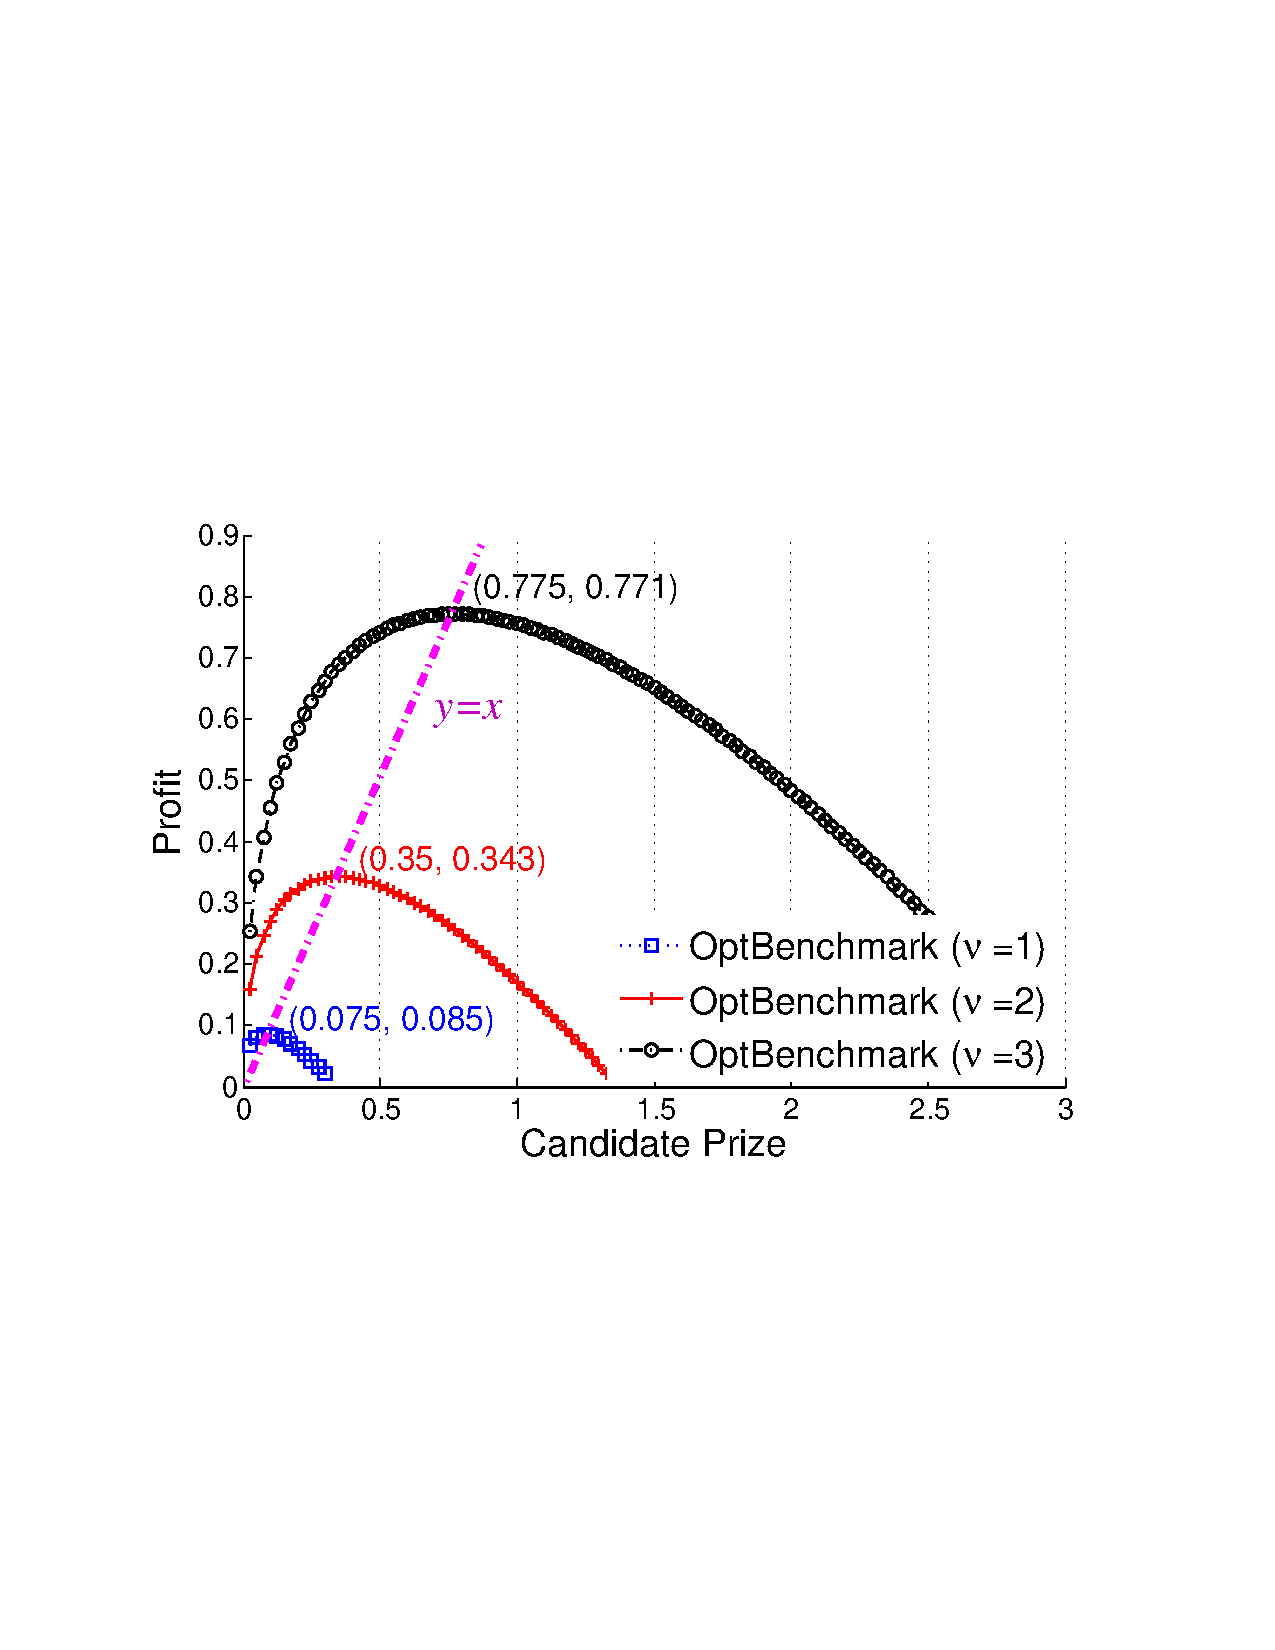
\includegraphics[trim=2.5cm 8.2cm 3.4cm 8.6cm,clip,width=\linewidth]{traject2.pdf}}
  \caption{OptBenchmark: Trajectory of finding the duple of optimal prize and maximum profit, annotated at the peak of each curve.}\label{fig:traject}
\endminipage\hfill
\minipage{0.3\textwidth}
  \fbox{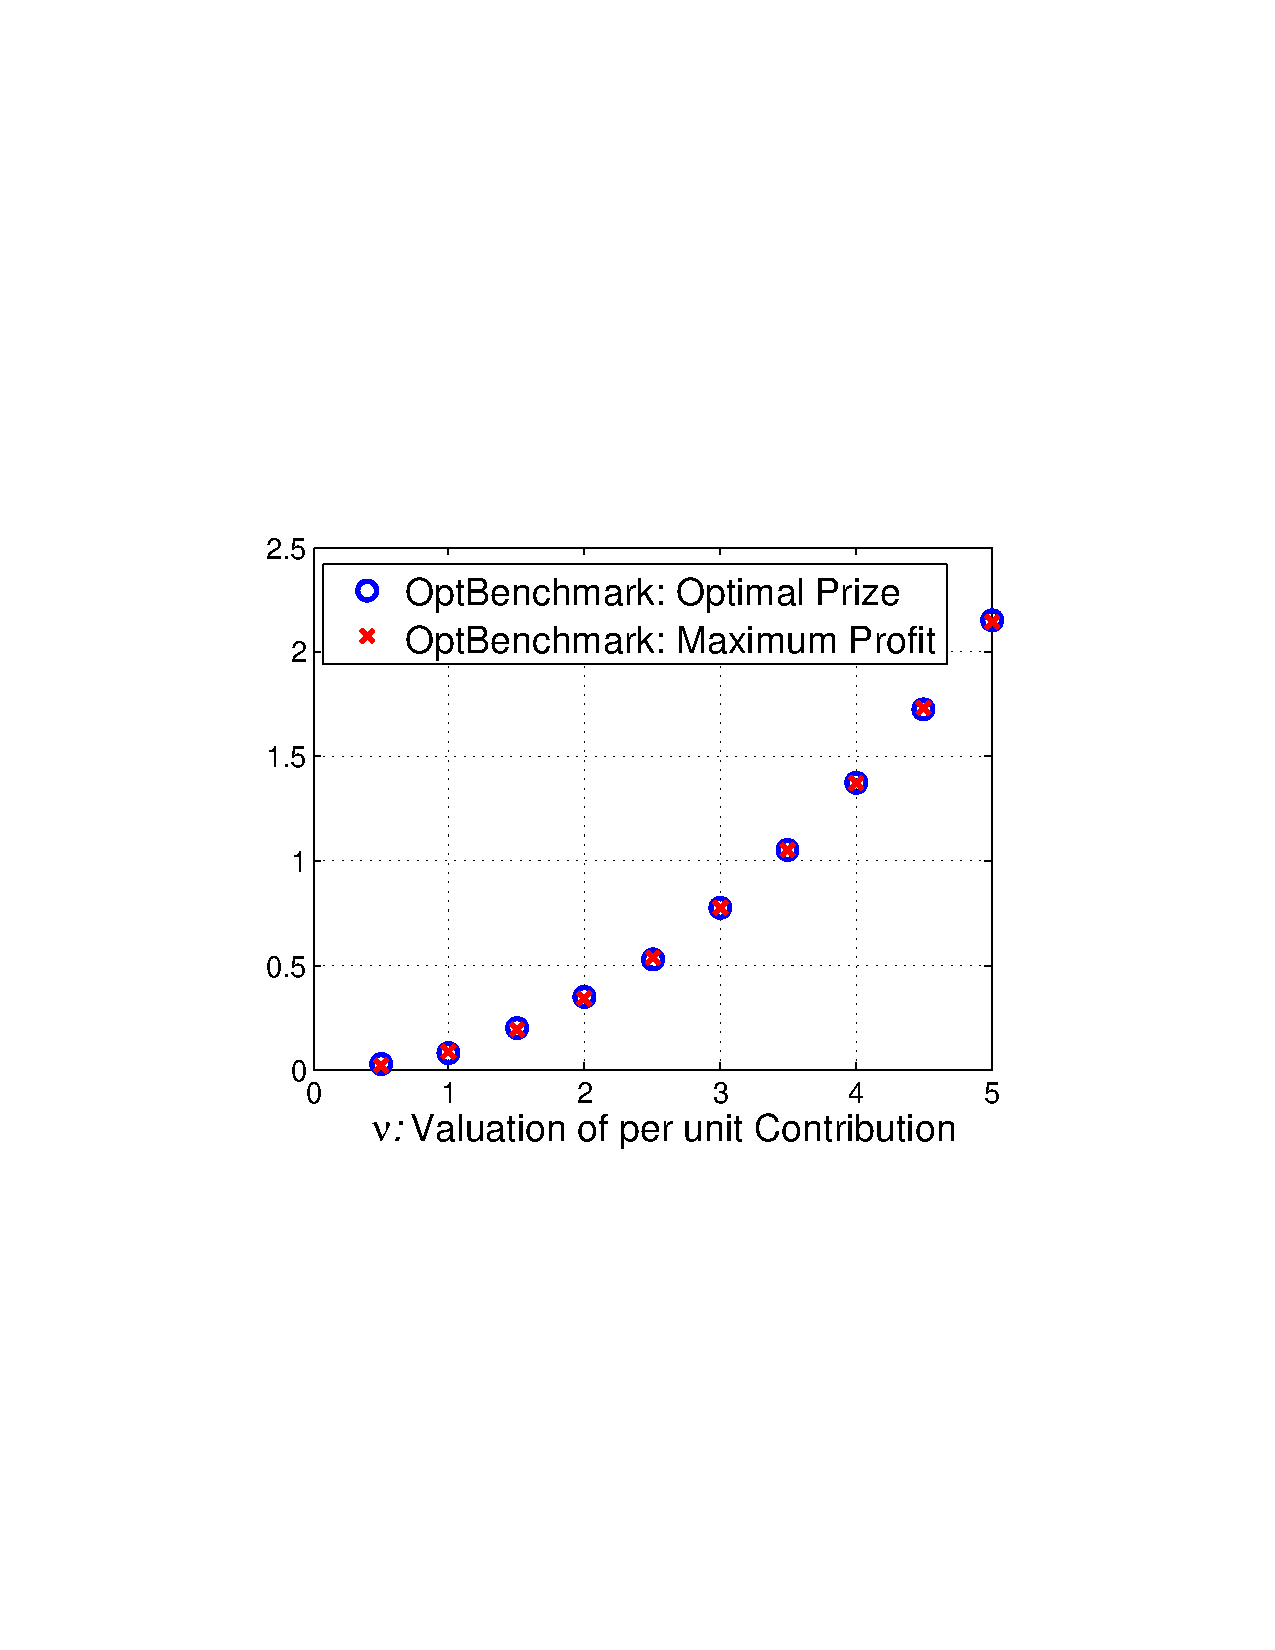
\includegraphics[trim=4.4cm 8.5cm 4.5cm 9cm,clip,width=\linewidth]{pp-vs-nu2.pdf}}
  \caption{OptBenchmark: Impact of $\nu$ on prize and profit.}\label{fig:pp-vs-nu}
\endminipage
\setcounter{figure}{3}
\minipage{0.31\textwidth}%
  \fbox{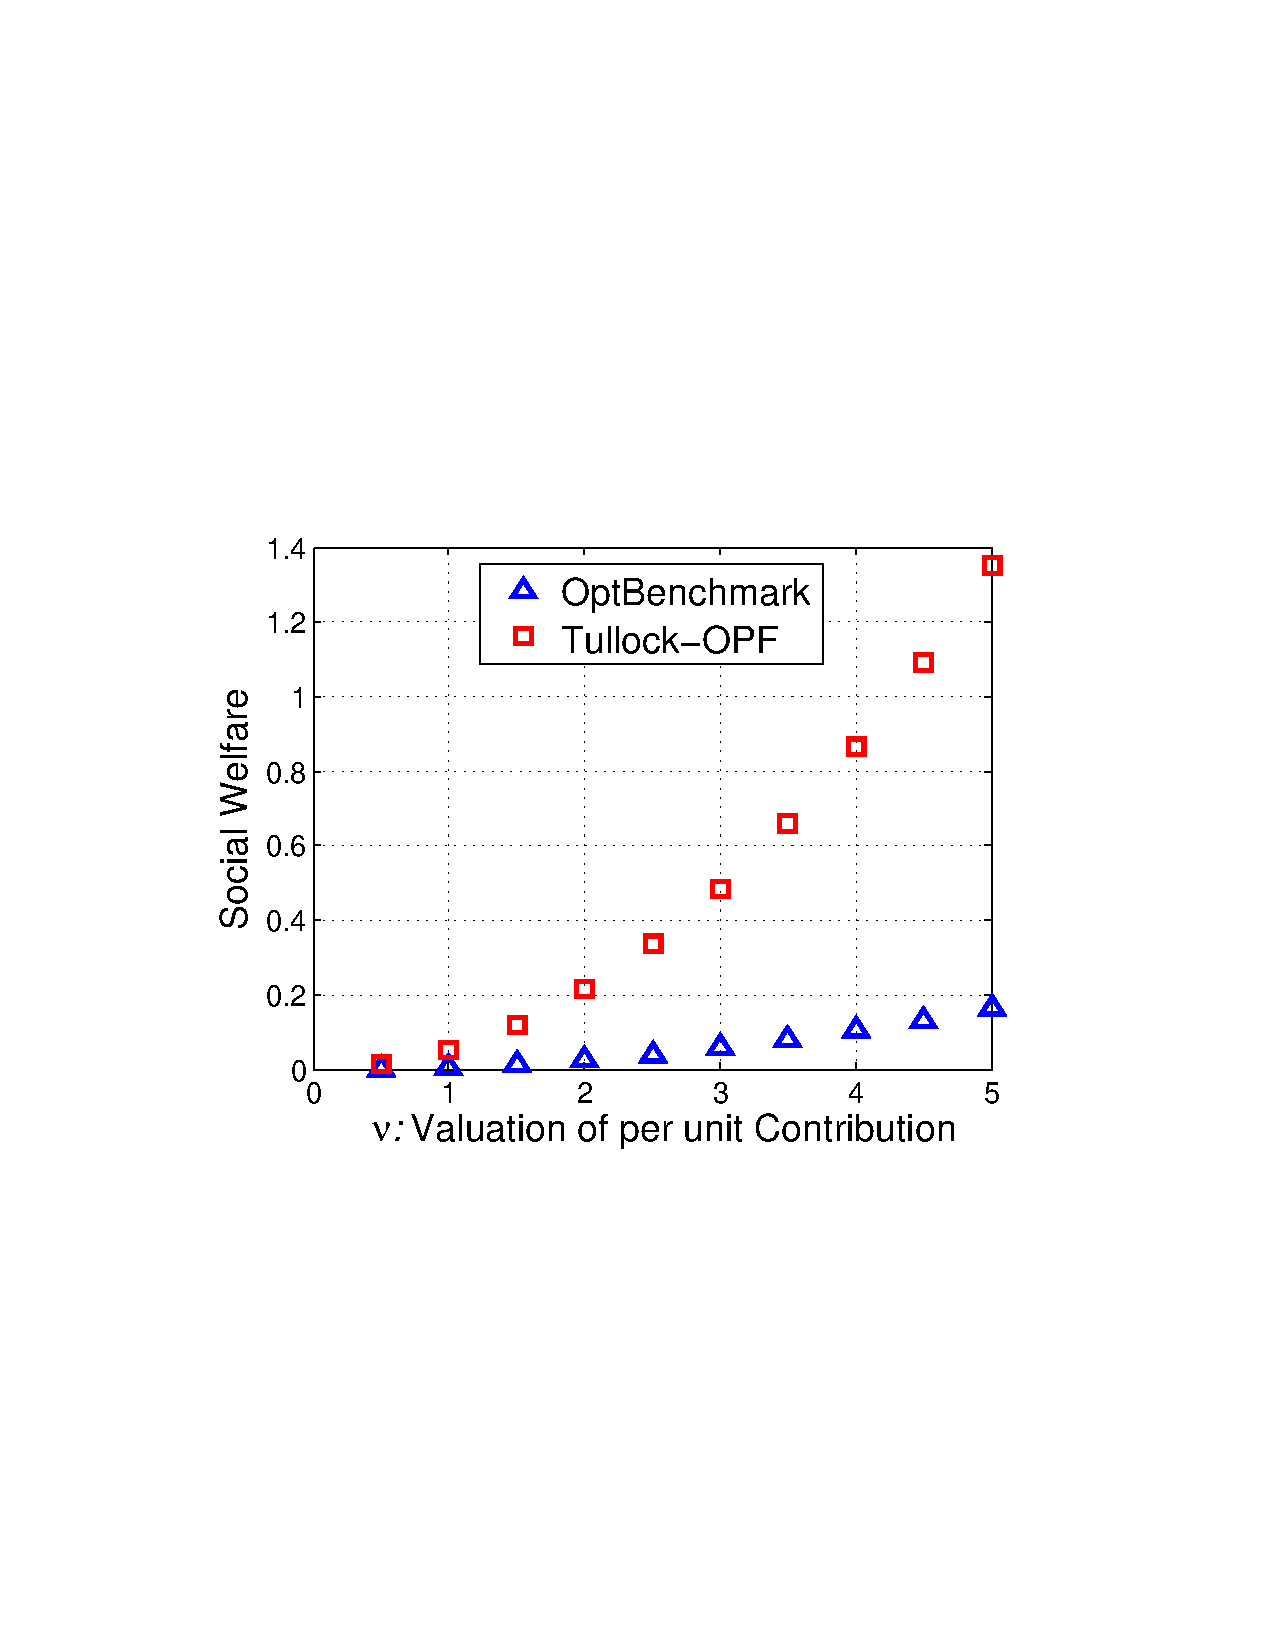
\includegraphics[trim=3.6cm 8.5cm 4.5cm 9cm,clip,width=\linewidth]{socwf2.pdf}}
  \caption{Comparison of Tullock-OPF against OptBenchmark: Social Welfare.}\label{fig:socwf}
\endminipage
\end{figure*}


\subsection{Comparison}
Given that both Tullock-OPF and OptBenchmark are solved by now, we proceed to compare them with respect to the four metrics mentioned earlier.

\setcounter{figure}{2}
\begin{figure*}[tb]
\centering
\subfloat[Revenue: Equilibrium contribution strategy. Out of the $m$=100 quadrature points, only 20 are shown for better visibility.]{\label{fig:strategy}
\fbox{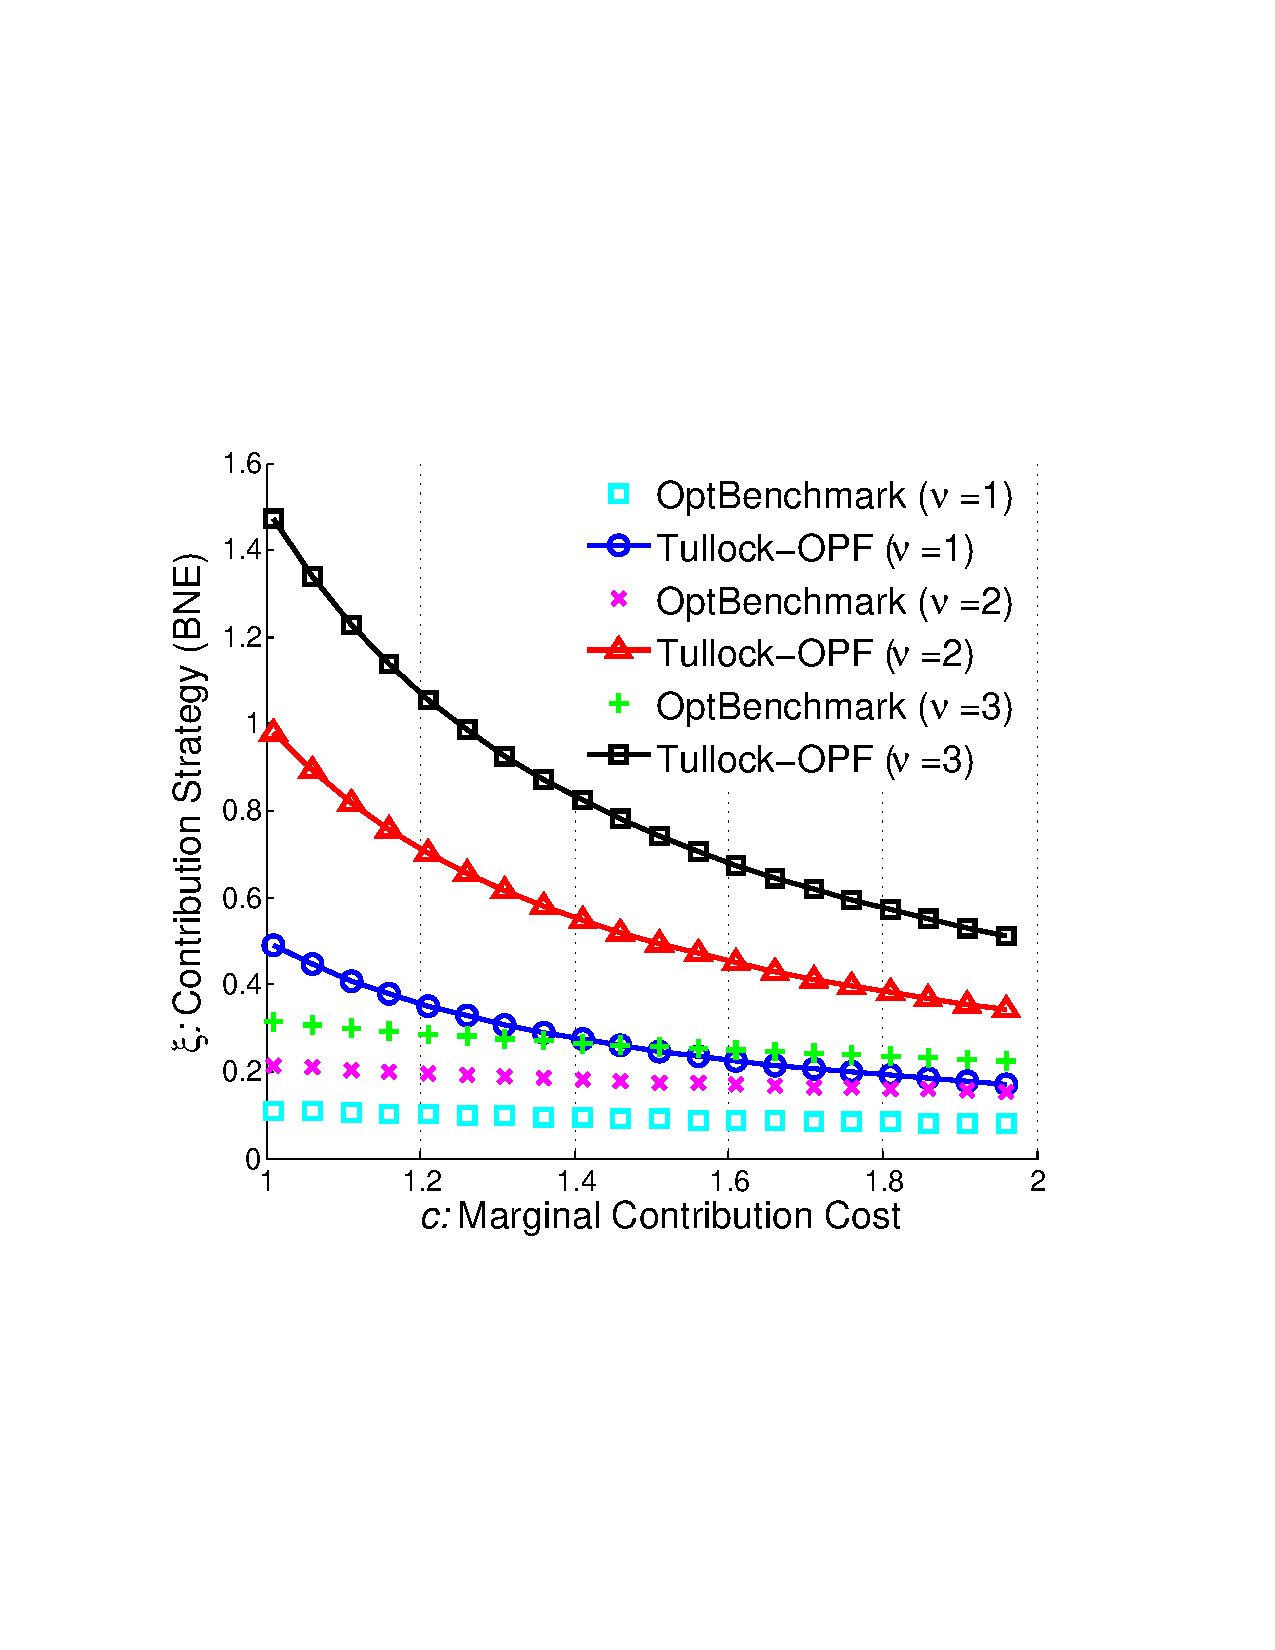
\includegraphics[trim=2.8cm 6.9cm 3.7cm 7.3cm,clip,width=0.3\linewidth]{strategy2.pdf}}}\hfil
\subfloat[Cost: Prize. Note that the support of Tullock-OPF is ${\xi\in[\nu/6,\nu/2]}$.]{\label{fig:prize}
\fbox{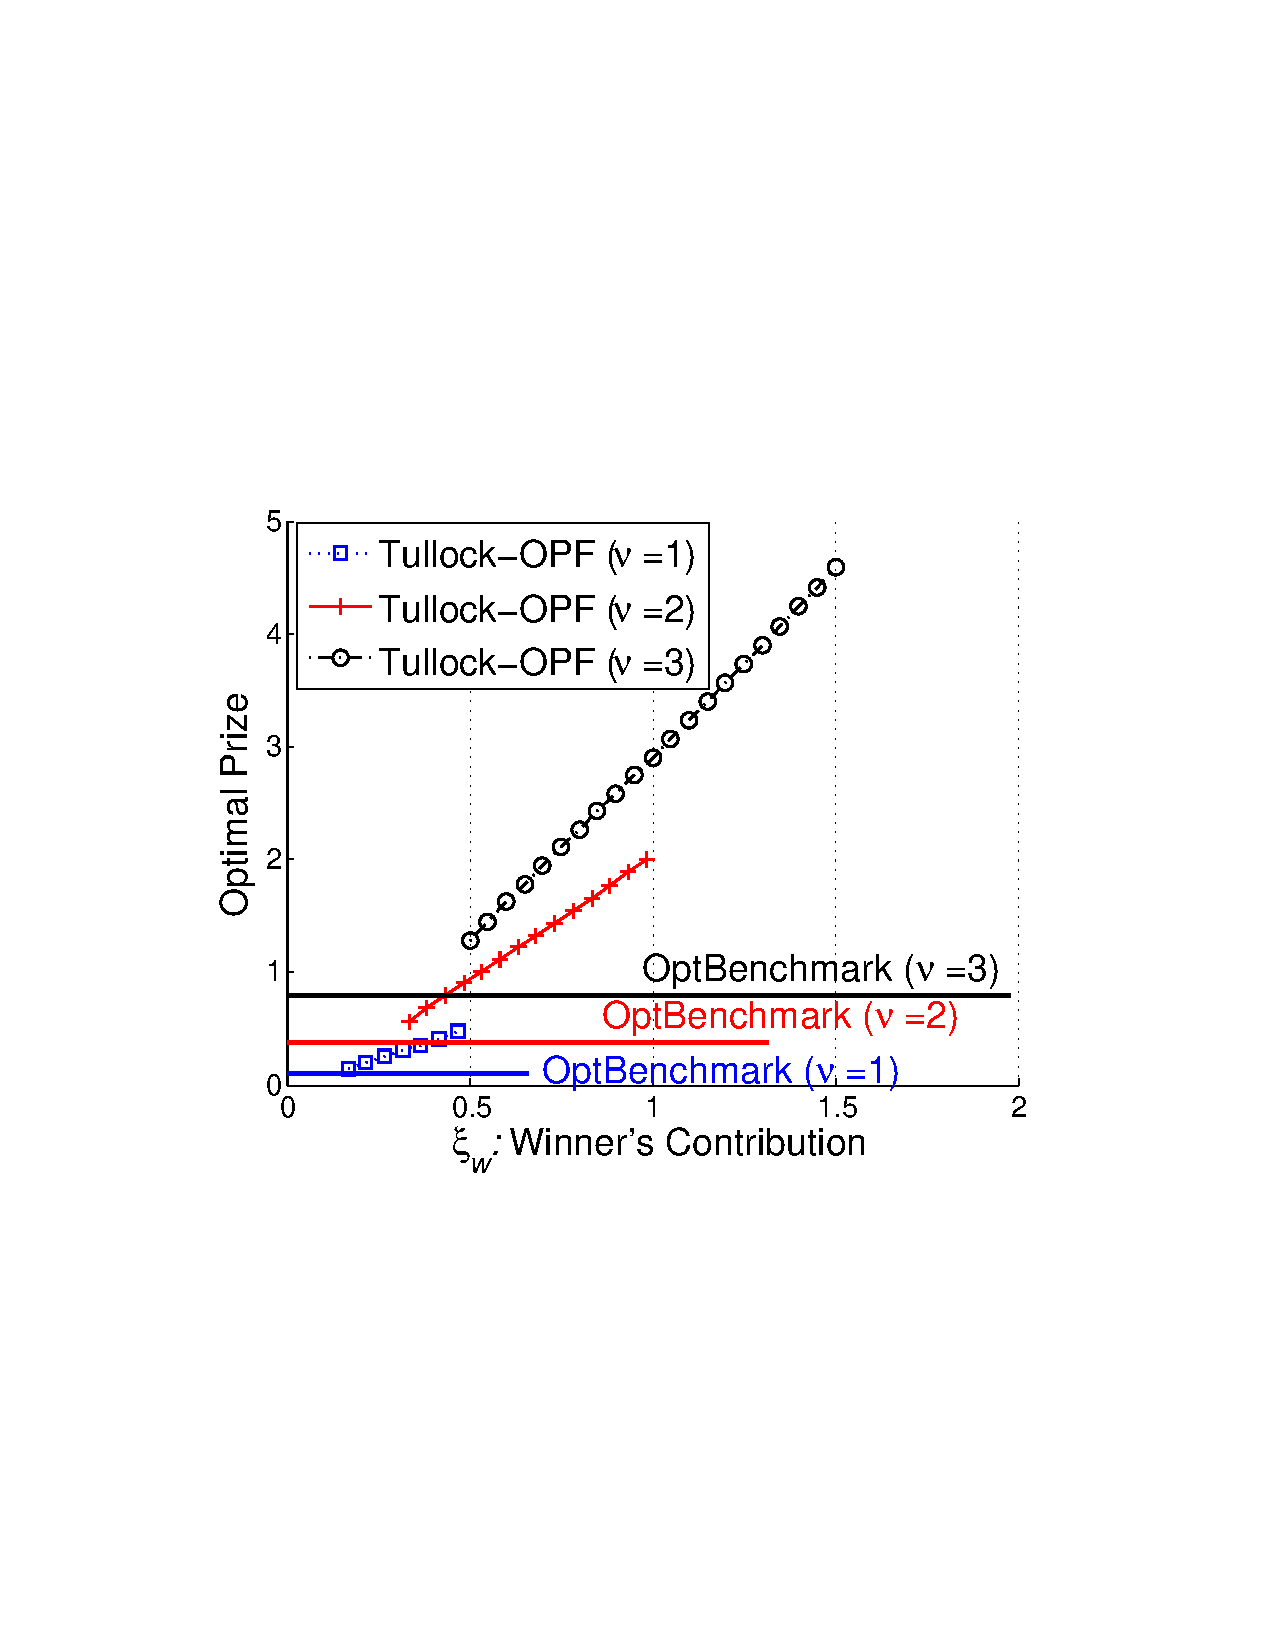
\includegraphics[trim=3.5cm 8cm 4cm 8.4cm,clip,width=0.32\linewidth]{prize2.pdf}}}\hfil
\subfloat[Profit.]{\label{fig:profit}
\fbox{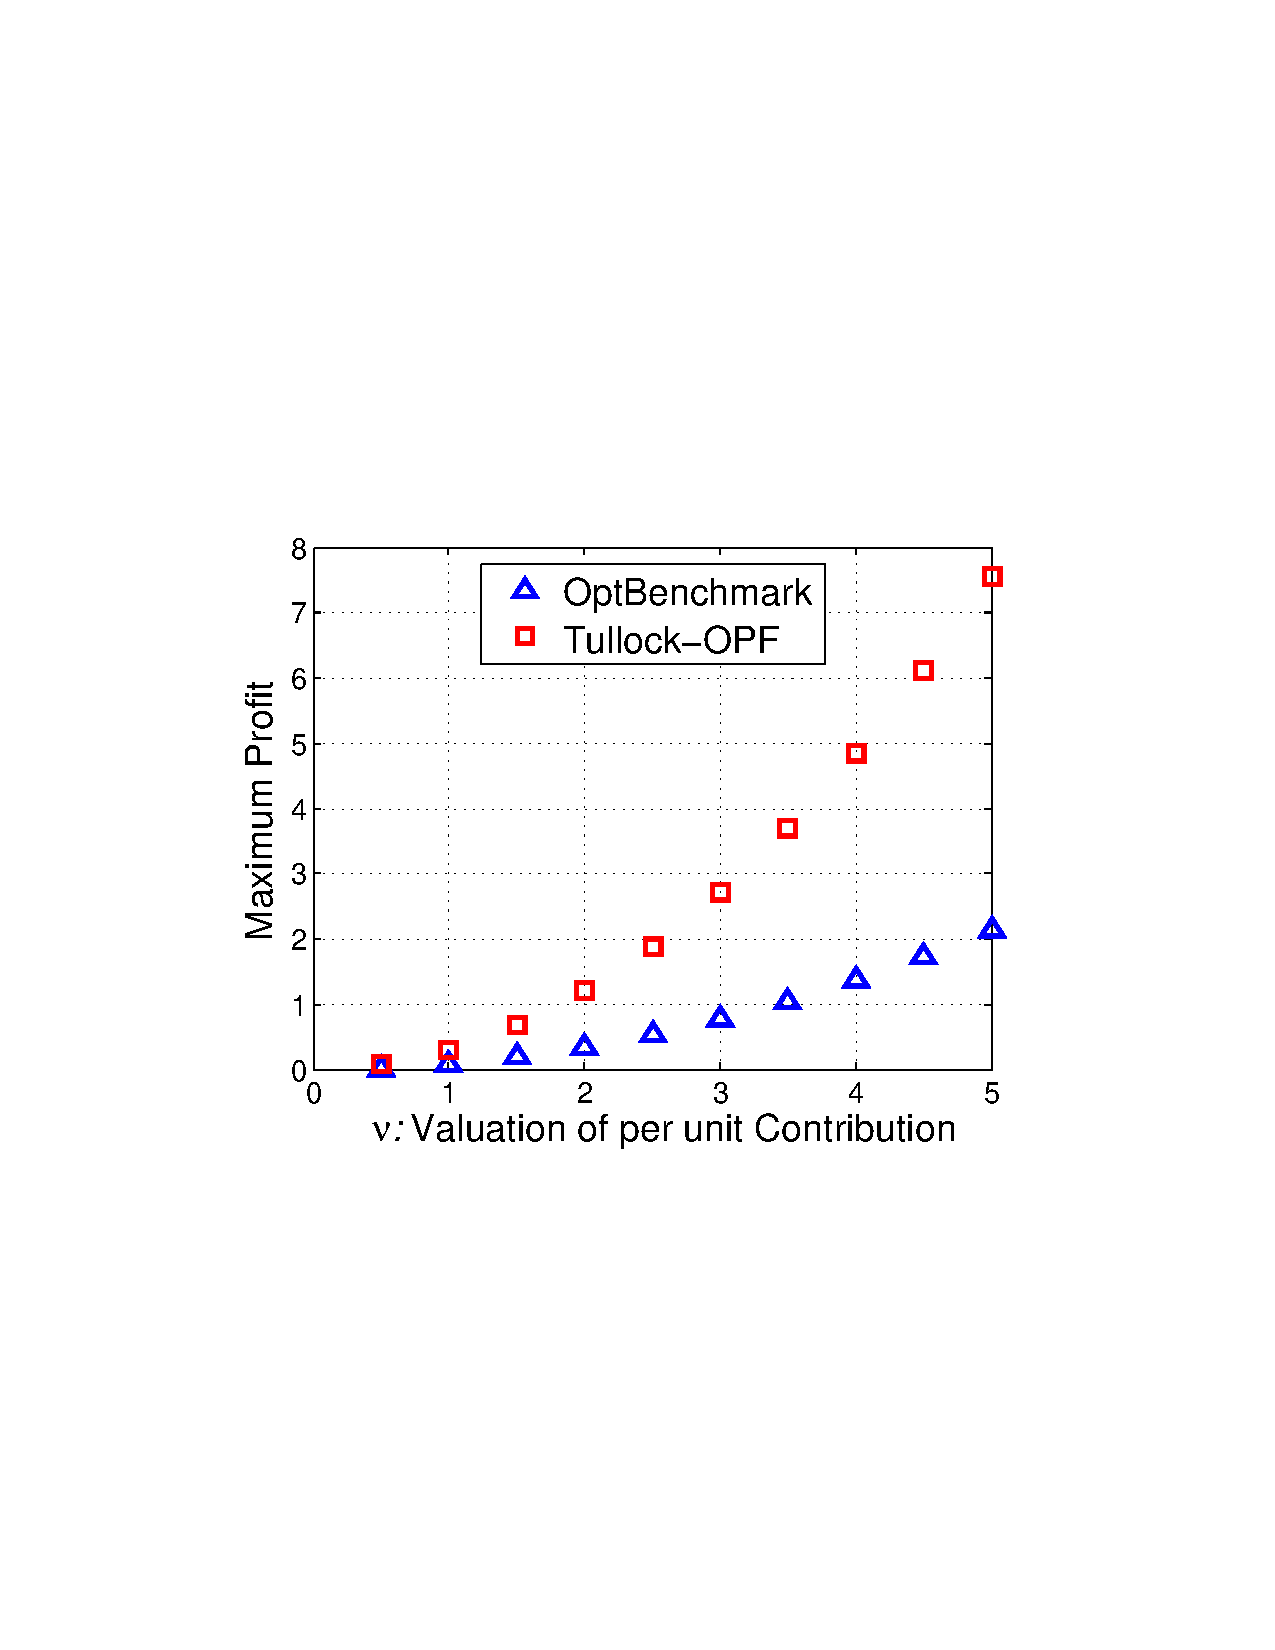
\includegraphics[trim=4cm 8.4cm 4.5cm 9cm,clip,width=0.325\linewidth]{profit2.pdf}}}
\caption{Comparison of Tullock-OPF against OptBenchmark.}
\label{fig:compare}
\end{figure*}

{\bf Crowdsourcing Revenue}: \fref{fig:strategy} examines the equilibrium contribution strategy of players as a function of player type, for each $\nu=1,2,3$. We remark on three observations. First, in all the cases (3$\times$2 curves), the strategy is monotone decreasing in type, which conforms to our \pref{thm:exists} (which subsumes $V(\cdot)$ being constant). The convex trend is also consistent with the literature: for example, we verified a special case of OptBenchmark with $h(\xi)=\xi$, $\nu=1$, $c\in[0.01,1.01]$, which is the same as \cite{Fey08}, and the result (not reproduced here) exactly matched \cite{Fey08}. Second, for any $\nu$, Tullock-OPF elicits significantly higher contribution than OptBenchmark for every possible type $c$, by about 150\% for high-cost (weak) players and 400\% for low-cost (strong) players. Third, in both mechanisms, the highest-cost or weakest player makes strictly positive contribution, i.e., $\uline\xi=\beta(\ovl c)>0$, indicating a sheer contrast between Tullock contests and auctions where $\uline\xi=0$; here we recall the first remark below \thmref{thm:optimal}.

{\bf Crowdsourcing Cost}: \fref{fig:prize} compares the optimal prize function $V^*(\xi_w)$ in Tullock-OPF against the optimal fixed prize $V_0^*$ in OptBenchmark. Note that the support of $V^*(\xi_w)$ is $[\uline\xi,\ovl\xi]=[\nu/6,\nu/2]$ which follows from \eqref{eq:opf-strategy}. While it is intuitive that each of the three $V^*(\xi_w)$ curves increases in winner's contribution, it is interesting to note that each curve fits a straight line very well, which suggests that the computation of \eqref{eq:opf-prize} could be remarkably simplified in practice via linear approximation. While this advantage should not be overstated as to how it generalizes, it hints at a possible line of future work. Moreover and noteworthily, the diagram shows that the prize offered by Tullock-OPF is generally well above OptBenchmark. This raises an important question that whether this much higher cost to be borne by the crowdsourcer will eventually pay off, which is answered next.

{\bf Crowdsourcing Profit}: \fref{fig:profit} evaluates the maximum profit that a crowdsourcer garners from the two mechanisms. The salient observation is that Tullock-OPF outperforms OptBenchmark by a large profit margin, which strongly corroborates our proposal of using an optimized prize function to supersede the conventional, fixed prize in Tullock contests. For a closer examination, we collate the results into \tref{tab:profit} and calculate the ratio between each pair of profits for all the $\nu$'s. It is interesting to note that the ratio almost remains constant, at about 3.53. This could be explained by the nature of optimization which has pushed the profit to the limit in both mechanisms. In addition, a rigorous analysis as well as investigating to what extent this result can generalize may be worth future exploring.
\begin{table*}[ht]
\caption{Profit Comparison and Ratios}\label{tab:profit}
\centering
\begin{tabular}{l | c | c | c | c | c | c | c | c | c | c } \hline\hline 
{\bf $\nu$} & 0.5 & 1 & 1.5 & 2 & 2.5 & 3 & 3.5 & 4 & 4.5 & 5 \\ \hline 
{\bf OptBenchmark} &  0.0213 & 0.0853 & 0.1927 & 0.3426 & 0.5354 & 0.7710 & 1.0494 & 1.3707 & 1.7347 & 2.1417 \\ \hline
{\bf Tullock-OPF} &  0.0756 & 0.3024 & 0.6805 & 1.2097 & 1.8902 & 2.7219 & 3.7048 & 4.8389 & 6.1242 & 7.5608 \\ \hline
{\bf Ratio} &  3.5533 & 3.5450 & 3.5315 & 3.5307 & 3.5306 & 3.5303 & 3.5303 & 3.5303 & 3.5303 & 3.5303 \\ \hline\hline
\end{tabular}
\end{table*}

{\bf Social Welfare}: In Tullock-OPF, this can be analytically obtained. To solve for $U = \mathbbm E_{\vect c}[\sum_{i=1}^n u_i]$, rather than using the definition \eqref{eq:ut}, we leverage on \lref{lem:strategy} which lends us much more convenience:
\begin{align}
U &= \mathbbm E_{\vect c}\left[\sum_{i=1}^n u_i\right] = n \int_{\uline c}^{\ovl c} \int_{c}^{\ovl c} h(\beta(\tilde c)) \opd \tilde c \opd F(c) \label{eq:socwf}\\
&= n \int_{\uline c}^{\ovl c} \int_{c}^{\ovl c} \frac{\nu^2}{(4\tilde c -2)^2} \opd \tilde c \opd F(c) \nn\\
&= 2 \int_1^2 \frac{\nu^2}{8} \left(\inv{2c-1} - \inv 3\right) \opd c 
= \left(\frac{\log 3}{8} - \inv{12}\right) \nu^2 \nn
\end{align}

One the other hand, the social welfare in OptBenchmark has to resort to numerical methods. To do so, we take the output $\vect\Xi_0^*$ of \aref{alg:opt-fixed}, and denote the row $\vect\Xi_{0}^*(\nu)$ corresponding to each $\nu$ by a strategy profile $\vect\xi_{0}^*$. Thus, we can compute the social welfare as
\begin{align}
U_0 = n \Delta_m \sum_{i=1}^m \left[ f(c_i)
\left( \Delta_m \sum_{j=i}^m {\xi_{0j}^*}^2 \right) \right],
\end{align}
which can be understood by rewriting \eqref{eq:socwf} as
\[ U = n \int_{\uline c}^{\ovl c} f(c) \int_{c}^{\ovl c} \xi^2 \opd \tilde c \opd c \]
and noting that \lref{lem:strategy} applies, without change, to fixed-prize cases where $V(\cdot)$ is a constant.

The results are presented in \fref{fig:socwf}. The observation is exciting: Tullock-OPF outstrips OptBechmark in an even more striking manner as compared to profit in \fref{fig:profit}. The detailed data are collated in \tref{tab:socwf}, which indicates a remarkable improvement of 7--9.3 folds. On the other hand, the nearly constant ratio in \tref{tab:profit} is not duplicated here.


\begin{table*}[ht]
\caption{Social Welfare Comparison and Ratios}\label{tab:socwf}
\centering
\begin{tabular}{l | c | c | c | c | c | c | c | c | c | c } \hline\hline 
{\bf $\nu$} & 0.5 & 1 & 1.5 & 2 & 2.5 & 3 & 3.5 & 4 & 4.5 & 5 \\ \hline 
{\bf OptBenchmark} & 0.0019 & 0.0058 & 0.0155 & 0.0271 & 0.0407 & 0.0600 & 0.0813 & 0.1065 & 0.1336 & 0.1666 \\ \hline
{\bf Tullock-OPF} & 0.0135 & 0.0540 & 0.1215 & 0.2160 & 0.3375 & 0.4859 & 0.6614 & 0.8639 & 1.0934 & 1.3498 \\ \hline
{\bf Ratio} & 6.9693 & 9.2924 & 7.8404 & 7.9649 & 8.2968 & 8.0934 & 8.1308 & 8.1097 & 8.1813 & 8.1038 \\ \hline\hline
\end{tabular}
\end{table*}

It may be puzzling as to why the crowdsourcer can reap higher profit while, at the same time, users altogether also gain higher surplus. This constitutes a ``win-win'' situation which is highly desirable but typically hard to attain. To explain this, we note the following rationales. First, generally speaking, crowdsourcing is not a {\em zero-sum game} like the stock market; rather, it involves a {\em wealth creation} process in which users exert effort to create ``something'' valuable that we have abstracted as ``contribution''. Second, there exists a {\em value asymmetry} between players and the crowdsourcer, where the crowdsourcer typically values contribution higher than players do. This value asymmetry is a common phenomenon in reality: for example in the worldwide emerging Smart City and Smart Nation initiatives nowadays, citizen-generated data such as ambient noise and GPS traces collected by smartphones do not usually bear much value to the phone owners but can be very valuable to a crowdsourcer such as a noise control bureau or a transport company (like Waze). Thus, it makes perfect business sense for a crowdsourcer to provision certain attractive reward to incentivize more user contribution which in turn bears even more value to the crowdsourcer.

\subsection{Impact of Crowdsourcer's Valuation}\label{sec:orgvalue}

Recall that we have introduced a new parameter, $\nu$, to our model in \sref{sec:model} (cf. \eqref{eq:orgut-def}). Herein, we investigate how it affects the various performance indicators.

This effect is explicitly examined with respect to the optimal fixed prize (\fref{fig:pp-vs-nu}), maximum profit (\fref{fig:profit}), and social welfare (\fref{fig:socwf}), where it is clearly shown that the impact of $\nu$ on these three metrics is {\em nonlinear} (convex). Furthermore, this effect is also implicitly examined with respect to the equilibrium contribution strategy (\fref{fig:strategy}) and optimal prize function (\fref{fig:prize}) (in both diagrams one needs to compare across different curves corresponding to different $\nu$'s),
and we see that the impact of $\nu$ on these two metrics is approximately {\em linear}. 

The main message conveyed here is that, if a crowdsourcer increases his valuation of user contribution, e.g. by improving his business processes to better exploit user contribution, his profit and the players' social welfare will both {\em increase faster}. This is an interesting finding uncovered due to our introduction of $\nu$. Moreover, this observation applies to both Tullock-OPF and the conventional case.

Now we dive in deeper to explain the correlation between the above nonlinearity and linearity. On the one hand, the case of OptBenchmark can be nicely explained: (a) the nonlinear profit (\fref{fig:profit}) results from the linear revenue (contribution; \fref{fig:strategy}) and nonlinear cost (prize; \fref{fig:pp-vs-nu}), and (b) the nonlinear social welfare (\fref{fig:socwf}) follows from the nonlinear prize (player's gain; \fref{fig:pp-vs-nu}) and the linear strategy (player's cost; \fref{fig:strategy}).

On the other hand, the case of Tullock-OPF is not that straightforward, since both revenue (contribution) and cost (prize) seem to be linear across different $\nu$'s. In fact, an overlooked fact was that the prize functions in \fref{fig:prize} are {\em shifted} horizontally, and thus one should compare prizes across $\nu$'s for the same {\em winner} rather than for the same amount of {\em contribution}. To do this, a simple way is to compare the maximum (or the minimum) winner contribution $\xi_w$ across different curves, as it can uniquely identify a particular winner. This reveals that the impact of $\nu$ on prize is actually {\em nonlinear}. Combined with the linearity on revenue (\fref{fig:strategy}), this explains why the profit and social welfare in Tullock-OPF are nonlinear in $\nu$. 

\subsection{$n$-Player Case}

In this section, we extend our investigation to $n$ players. We conjecture that the above comparison results will continue to hold in the $n$-player case, and hence we will not repeat the same comparisons. In fact, as Ryvkin \cite{Ryvkin10} pointed out, it is computationally infeasible to numerically solve fixed-prize Tullock contests for an arbitrary large number of players because of the ``curse of dimensionality''. Therefore, this section focuses on Tullock-OPF. In particular, we are interested in how the {\em composition} of a participant pool, i.e., the distribution of the player types, affects the two key metrics, profit and social welfare.

We consider two participant pools: {\it Population-1} draws player types from the same distribution as above, i.e., $F(c)=c-1, c\in[1,2]$, while {\it Population-2} draws from another distribution $G(c)=\frac{c}{2} -\inv 4, c\in[0.5,2.5]$. Thus, Population-2 is more {\em diverse}---or is more {\em uncertain} in player types---than Population-1,
while they statistically share the same mean value (1.5).


Following from \thmref{thm:optimal}, the equilibrium strategy in Population-2 is
$\xi_G = \frac{\nu}{4c - 1}$, and thus the maximum profit is
\begin{align}\label{eq:opf-profit-Gn}
\pi_{n,G}^* \! &=\! \frac{n}{2} \int_{0.5}^{2.5}\! \left[ 
\frac{\nu^2}{4c-1}\! - \!\frac{\nu^2 c}{(4c-1)^2}\! +\! 
(c-\inv 2) \Big(\frac{\nu^2}{81}\! - \!\frac{\nu^2}{(4c-1)^2}\Big) \right]\! \opd c \nn\\
&=\! \frac{n \nu^2}{2} \int_{0.5}^{2.5}\! \left( \inv{8c-2}\! +\! \frac{2c-1}{162} \right) \opd c
= \left( \frac{\log 3}{8} + \frac{2}{81} \right) n \nu^2. \nn 
\end{align}
For Population-1, we leverage \eqref{eq:opf-profit} as a shortcut to obtain
\begin{align}
\pi_{n,F}^* = \left( \frac{\log 3}{8} + \inv{72} \right) n \nu^2.
\end{align}
Social welfare can be solved by referring to \eqref{eq:socwf}:
\begin{align*}
U^*_{n,G} &= \frac{n}{2} \int_{\uline c}^{\ovl c} \int_{c}^{\ovl c} \frac{\nu^2}{(4\tilde c -1)^2} \opd \tilde c \opd c
= \left(\frac{\log 3}{16} - \inv{36}\right) n \nu^2, \\
U^*_{n,F} &= \left(\frac{\log 3}{16} - \inv{24}\right) n \nu^2.
\end{align*}

Thus it immediately follows from the above that
\[  \pi_{n,G}^* > \pi_{n,F}^*, \quad U^*_{n,G} > U^*_{n,F}, \quad \forall n\ge 2, \forall \nu>0.\]
This tells that Population-2 is superior to Population-1 in terms of both profit and social welfare. An insight that may be drawn from this set of results is that population {\em diversity} or {\em uncertainty} is beneficial to Tullock-contest based crowdsourcing for both crowdsourcers and participants.


\section{Conclusion}\label{sec:conc}

To recap, this work has presented a first attempt to use Tullock contests as a new framework to design incentive mechanisms for crowdsourcing. Furthermore, we have explored a novel dimension in the space of optimal Tullock contest design, by superseding the conventional, fixed prize by an optimal prize function for utility maximization. In stark contrast to prior art, we have obtained an analytical solution to the unique Bayesian equilibrium, and found that the equilibrium is robust to an increasing number of rivals. As our model employs a very general contest success function and assumes incomplete information, the mechanism and results would fit a wide range of practical crowdsourcing applications.
For example, WiFiScout\cite{wifiscout14mass} is a mobile app that aims to profile the performance of citywide WiFi access points by eliciting personal experience on WiFi usage from smartphone users. Similarly, OpenSignal\cite{opensignal} aims to construct citywide 3G and 4G LTE cell coverage maps through crowdsourcing too.

The superiority of our design has been demonstrated through extensive evaluations by comparing against a fully-optimized benchmark. Constructing this optimal benchmark significantly extends prior art which only {\em solves} conventional, fixed-prize Tullock contests. This benchmark would be highly relevant to a wider research community for future performance evaluations.

Moreover, we have introduced the crowdsourcer's valuation of user contribution which further extends usual contest models (besides our prize function). It is shown to impact two key metrics---the crowdsourcer's profit and players' social welfare---in a nonlinear (exponential) manner, which bears practical implication on the worth of improving crowdsourcers' business processes. Therefore, this new parameter could be included by future studies (e.g., on radio spectrum auctions or heterogeneous networks) in mathematical models to capture {\em value asymmetry}
and uncover phenomena that are previously unseen.


\metacom{Ultimately, this paper opens up a completely new field of fundamental research in incentive mechanism design for crowdsourcing, using Tullock contests with a functionized prize.}



%\bibliographystyle{IEEEtran}
\bibliography{IEEEabrv}
%\documentclass[iop]{emulateapj}
\usepackage{graphicx, lmodern, dcolumn}
\usepackage[T1]{fontenc}
\usepackage[para,flushleft]{threeparttable}
\usepackage{amssymb,amsmath}
\newcommand{\lapprox }{{\lower0.8ex\hbox{$\buildrel <\over\sim$}}}
\newcommand{\gapprox }{{\lower0.8ex\hbox{$\buildrel >\over\sim$}}}

\shorttitle{Stellar Feedback in Galaxy Simulations}
\shortauthors{A. N\'u\~nez et al.}

\bibliographystyle{apj}
\begin{document}
\title{Modeling for Stellar Feedback in Galaxy Formation Simulations}
\author{Alejandro N\'u\~nez\altaffilmark{1}, Jeremiah P. Ostriker\altaffilmark{1,2}, Thorsten Naab\altaffilmark{3}, Ludwig Oser\altaffilmark{3}, Chia-Yu Hu\altaffilmark{3} and Ena Choi\altaffilmark{4}}

\altaffiltext{1}{Department of Astronomy, Columbia University, 550 West 120th Street, New York, NY 10027, USA}
\altaffiltext{2}{Princeton University Observatory, Princeton, NJ 08544, USA}
\altaffiltext{3}{Max-Planck-Institut f\"ur Astrophysik, Karl-Schwarzschild-Strasse 1, D-85741 Garching, Germany}
\altaffiltext{4}{Department of Physics and Astronomy, Rutgers, The State University of New Jersey, Piscataway, NY 08854, USA}

\begin{abstract}
Various heuristic approaches to model unresolved supernova (SN) feedback in galaxy formation simulations exist to reproduce the formation of spiral galaxies and the overall inefficient conversion of gas into stars. Some models, however, require resolution dependent scalings. We present a sub-resolution model representing the three major phases of supernova blast wave evolution ---free expansion, energy conserving Sedov-Taylor, and momentum conserving snowplow--- with energy scalings adopted from high-resolution interstellar-medium simulations in both uniform and multiphase media. We allow for the effects of significantly enhanced SN remnant propagation in a multiphase medium with the cooling radius scaling with the hot volume fraction, $f_{\mathrm{hot}}$, as $(1 - f_{\mathrm{hot}})^{-4/5}$. We also include winds from young massive stars and AGB stars, Str\"omgren sphere gas heating by massive stars, and a gas cooling limiting mechanism driven by radiative recombination of dense H\textsc{ii} regions. We present initial tests for isolated Milky-Way like systems simulated with the \textsc{Gadget} based code SPHgal with improved SPH prescription. Compared to pure thermal SN input, the model significantly suppresses star formation at early epochs, with star formation extended both in time and space in better accord with observations. Compared to models with pure thermal SN feedback, the age at which half the stellar mass is assembled increases by a factor of 2.4, and the mass loading parameter and gas outflow rate from the galactic disk increase by a factor of 2. Simulation results are converged for a two order of magnitude variation in particle mass in the range (1.3--130)$\times 10^4$ solar masses. 
\end{abstract}

\keywords{methods: numerical -- galaxies: formation -- galaxies: evolution -- galaxies: stellar content -- galaxies: abundances}

\section{Introduction}
Current cosmological simulations of baryonic and dark matter (DM) have made great advances in recreating the epochs and spatial distribution of galaxies \citep[see][for reviews]{Bertschinger98, Springel10, Somerville15}. A major challenge is the reproduction of the overall inefficiency of galaxy formation with physically self-consistent models. Typically, there is a tendency for gas in simulated galaxies to transform into stars too efficiently and too early, resulting in stellar mass fractions larger than observed and stellar populations older than observed \citep[e.g.,][]{White91, Keres09, Guo10, Moster13}.

In the case of low mass galaxies, early work has pointed at efficient feedback from supernova (SN) explosions as the appropriate solution, as it would suppress stellar formation at early epochs by heating up and diffusing gas, resulting in systems with lower stellar mass fractions and younger stellar ages \citep{White91}. The most widely used feedback is SN-driven outflows \citep{Dekel86, Larson74}, and such flows are detected in many observations at low and high redshifts \citep[e.g.,][]{Martin99, Strickland00, Rupke05, Steidel10, Newman12}. Considering the large variations in numerical implementations to create galactic outflows \citep[e.g.,][]{Springel03, Dubois08, Hopkins14, Dave13, Teyssier13, Vogelsberger14, Kimm2015, Schaye15, Simpson15} in galactic and cosmological simulations, it appears that it is not yet clear how best to implement SN feedback into simulations with limited resolution, which cannot fully resolve individual SN explosions and turbulent interstellar medium (ISM).

The simplest implementation of SN feedback is to inject thermal energy locally to the surrounding medium. This energy, however, is quickly radiated away in dense regions and the blast wave evolution is followed incorrectly \citep{Navarro93} \citep[see][for attempts to follow the blast wave evolution by turning off ``feedback'' or ``radiative losses'']{Stinson06}. This situation is an artifact of low resolution simulations, preventing previous SN explosions from vacating their surroundings, thus keeping subsequent SN explosions in dense areas \citep[see e.g.,][]{Dalla12, Kimm2015}. Some studies attempt to avoid this by applying a stochastic stellar feedback that is, first, calibrated to match the observed galaxy stellar mass function and, second, distributed over less mass than heating all neighbors, which results in longer cooling times \citep[see studies with the Evolution and Assembly of Galaxies and their Environments ---\textsc{Eagle}--- simulation, e.g.,][]{Schaye15, Furlong2015}.

A second order approach consists of transferring part or all of SN energy as kinetic energy to the surrounding medium by conserving momentum from the initial explosion \citep[see e.g.,][]{Dubois08b}. In this scenario, however, most of the energy transferred might still end up in thermal form, since the ratio of transferred kinetic energy to total SN energy is proportional to the ratio of transferred SN ejecta mass to the mass of the surrounding medium when momentum conservation is imposed \citep[see e.g.,][]{Hu14, Kimm2015}. Thus, while this approach explicitly includes the momentum of the ejecta, it effectively evolves to the usual ``thermal feedback'' algorithm. Therefore, overcooling still plays a part in hindering SN energy feedback from noticeably affecting the structure and evolution of simulated galaxies.

To prevent overcooling from nullifying SN energy feedback, recent studies adopted approximate approaches, such as decoupling SN-affected gas from hydrodynamic interactions \citep[e.g.,][]{Springel05a, Oppenheimer08, Vogelsberger13, Vogelsberger14}, implementing decoupled multi-phase ISM \citep{Scannapieco06, Aumer13}, suppressing radiative cooling effects on SN-heated gas for several tens of Myr \citep{Stinson06, Guedes2011}, constructing feedback mechanisms based on the evolution of superbubbles \citep{Keller2014, Keller2015}, and stochastically enhancing heating of SN-affected gas \citep{Dalla12, Schaye15}. As encouraging as the results are at replicating SN-driven winds and star formation rates (SFR), the methods have limited predictive power as they are not based on \emph{ab initio} physical modeling of the stellar feedback process.

In this study we attempt to develop a numerical stellar feedback prescription based as closely as possible on standard physical principles. It includes winds and heating from young massive stars as well as feedback from SN explosions, the latter following the known physical processes that govern the different phases of SN remnants. We use the smoothed particle hydrodynamics (SPH) code SPHGal \citep{Hu14}, an implementation that incorporates several improvements into the \textsc{Gadget} code \citep{Springel05b} to address some known SPH problems. Our approach is most similar to the stellar feedback in \citet{Agertz13} and \citet{Agertz2016}, as well as the Feedback in Realistic Environment (\textsc{Fire}) project, presented in \citet{Hopkins14} and used by \citet{Hopkins12, Hopkins2013b}, \citet{Muratov15}, and \citet{Su2016}. We apply our stellar feedback to an isolated Milky Way-like galaxy within an isolated dark halo. The tools developed here are in use by the cosmological code in \citet{Choi2016}.

We break our approach into three parts: feedback from young, pre-SN stars, feedback from dying low-mass stars, and feedback from SN events. (1) We include the effects of stellar winds from young stars by transferring momentum to neighboring gas particles for the first few Myr. We also heat gas particles within the Str\"omgren sphere of young star particles, mimicking the effects of ionizing radiation from massive stars \citep[see e.g.,][]{Renaud13}. (2) We transfer momentum from old, low-mass stars to the surrounding gas throughout several Gyr after a type II SN has occurred, to imitate the slow winds from asymptotic giant branch (AGB) stars.

(3) In our SN feedback model, we transfer SN energy to the closest gas particles to the SN event, each one receiving mass and energy according to a computed high resolution evolution of SN remnants (SNR). Detailed, very high resolution hydrodynamic simulations of SNR evolution \citep[see][for details and a review]{Li15} show that they pass through three successive phases: free expansion (FE), energy-conserving Sedov-Taylor (ST), and momentum-conserving snowplow (SP) \citep[see also][]{Kim15, Martizzi15, Walch15}. In our model, which we call the SP-model, each neighboring gas particle receives energy following the physics governing the SNR phase in which the gas particles lie. If the gas particle lies within the radius of the ejecta-dominated FE phase, SN energy is transferred by conserving the ejecta momentum. If the gas particle lies outside the FE radius but within the radius of the adiabatic blast wave ST phase, SN energy is transferred 30\% as kinetic energy and 70\% as thermal energy. Finally, if the gas particle is beyond the ST radius and into the realm of the pressure driven and momentum conserving SP phase \citep{Chevalier74}, then part of the original SN energy is dissipated and only a fraction is transferred to the gas particle, with the thermal portion dissipating more quickly than the kinetic portion following a prescription based on the detailed, high resolution, hydrodynamic treatments of SNR evolution in \citet{Li15}. Our treatment of feedback in the SP phase allows for a multi-phase medium by allowing for the volume fraction that is hot and tenuous.

The paper is organized as follows: in Sec.~\ref{sec:sim} we describe our numerical code simulation setup and feedback implementation, in Sec.~\ref{sec:results} we present our results, and in Sec.~\ref{sec:conclusions} we discuss these results and possible further developments.

\section{Simulations}\label{sec:sim}
\subsection{Numerical Code}\label{subsec:code}
To test our SN feedback treatment, we used a recently modified version of \textsc{Gadget} \citep{Springel05b}. The improved version ---SPHGal--- is described in detail by \citet{Hu14}. SPHGal includes an artificial viscosity implementation modified from the version presented in \citet{Cullen10} that uses a shock indicator based on the time derivative of the velocity divergence so as to improve the shock treatment. It also includes an energy diffusion implementation based on \citet{Read12} to correct for mixing instabilities. Finally, it includes a switch from a density--entropy to a pressure--entropy formulation to more accurately compute contact discontinuities as described in \citet{Hopkins2013a}, \citet{Ritchie01}, and \citet{Saitoh13}. As in the original \textsc{Gadget} code, SPHGal calculates the gas dynamics using the Lagrangian SPH technique \citep[see e.g.,][]{Monaghan92} and it ensures the conservation of energy and entropy \citep{Springel02}.

To complement the original \textsc{Gadget}, in which star formation and cooling was computed for a primordial composition of hydrogen and helium \citep{Katz96}, we included metal-line cooling using the method and cooling rates described in \citet{Aumer13}, where net cooling rates are tracked for 11 species: H, He, C, Ca, O, N, Ne, Mg, S, Si, and Fe. This method exposes the gas to the redshift-dependent UV/X-ray and cosmic microwave background modeled in \citet{Haardt01} and allows for mixing and spreading of metal abundances in the enriched gas. The code assumes the gas to begin with zero metallicity and to be optically thin and in ionization equilibrium.

\subsection{Star Formation Model}\label{subsec:sfr}
We included a chemical evolution and stochastic star formation model \citep{Aumer13} that considers enrichment by type II SNe, type Ia SNe, and AGB-type winds following the chemical yield prescriptions of \citet{Woosley95}, \citet{Karakas10}, and \citet{Iwamoto99}, respectively (see Secs.~\ref{subsubsec:implementation}--\ref{subsec:AGB}). As described in \citet{Aumer13}, SFR is set by $d\rho_*/dt = \varepsilon \rho\mathrm{_{gas}}/t\mathrm{_{dyn}}$, where $\rho_*$ and $\rho\mathrm{_{gas}}$ are the stellar and gas densities, respectively, $\varepsilon$ is the star formation efficiency, and $t\mathrm{_{dyn}}$ = $1/\sqrt{4\pi G\rho\mathrm{_{gas}}}$ is the local dynamical time for the gas particle. This is applied to gas particles in a convergent flow that are denser than a density threshold $\rho_{\mathrm{th}}$, which we define as
\begin{equation}\label{rhothresh}
  \rho_{\mathrm{th}} = \rho_0 \left(\frac{T_{\mathrm{gas}}}{T_0}\right)^3 \left(\frac{M_0}{M_{\mathrm{gas}}}\right)^{2},
\end{equation}
where $\rho_0$ is a critical threshold density value, $T_0$ is a critical temperature threshold, $M_0$ is a low-resolution particle mass fiducial value, and $T_{\mathrm{gas}}$ and $M_{\mathrm{gas}}$ are the temperature and mass of the gas particles, respectively. The values of $\rho_0$, $T_0$, and $M_0$ used in our simulations are listed in Table~\ref{table:params}. This scaling is modeled on the requirement that the density must exceed the value for the Jeans gravitational instability of a mass $M_{\mathrm{gas}}$ at temperature $T_{\mathrm{gas}}$. Star particles are then created stochastically with one gas particle being turned into one star particle of the same mass.

\subsection{Radiative Recombination}\label{subsec:recombination}
To account for radiative recombination processes in the cool ($\lapprox$10$^4$ K) ISM, where H and He line cooling dominate, we implemented a simple cooling limiting mechanism based on the recombination time of dense H\textsc{ii} regions. The recombination time for a gas particle is defined by $t_{\mathrm{rec}}^{-1} = n_{\mathrm{H}}\ \alpha_{\mathrm{B}}$, where $n_{\mathrm{H}}$ is the hydrogen number density of the ISM in cm$^{-3}$ and $\alpha_{\mathrm{B}}\approx2.56\times 10^{-13}$ cm$^3$ s$^{-1}$ is the effective radiative recombination rate for hydrogen, assuming a sphere temperature of $10^4$ K \citep{Draine11}.

We calculate the gas temperature resulting from the cooling limiting effect at every time step using the following definition
\begin{equation}\label{Trec}
  T_{n+1,\mathrm{rec}} = T_n + \frac{\Delta t}{\Delta t + t_{\mathrm{rec}}}(T_{n+1} - T_n),
\end{equation}
where $T_n$ and $T_{n+1}$ are the gas particle temperatures as determined by the cooling rates described in \citet{Aumer13} (see Sec.~\ref{subsec:code}) for the previous and current time steps $n$ and $n+1$, respectively, and $\Delta t$ is the time step size. If the resulting recombination-limited temperature $T_{n+1,\mathrm{rec}}$ is below $10^4$ K, then the gas particle gets assigned $T_{n+1,\mathrm{rec}}$ instead of $T_{n+1}$. The purpose of this limitation on the cooling rate is to allow for the fact that the relevant atomic processes (i.e., H and He line cooling) cannot proceed faster than the recombination time even if the code assumes (for simplicity) equilibrium states of ionization.

\subsection{Early Stellar Feedback}\label{subsec:youngfb}
As described by several stellar evolution models \citep[e.g.,][]{Leitherer99}, almost as much momentum is emitted into the ISM by winds from young massive stars as by type II SN explosions. Furthermore, radiation from these massive stars heats and ionizes the surrounding gas. The effect of this ionizing radiation can be characterized by the Str\"omgren sphere \citep{Stromgren39} surrounding massive stars, within which the ISM is ionized and heated to $\approx$10$^4$ K \citep{Hopkins12, Renaud13}.

\citet{Stinson13} presented an ``early stellar feedback'' model that adds thermal energy to gas surrounding stars, but only considering the energy in the UV stellar flux ---approximately 10\% of the total stellar luminosity \citep{Leitherer99}. To have a more complete model for pre-SN stellar feedback, we included two distinct feedback mechanisms from young massive stars before they explode as SN: stellar winds and Str\"omgren sphere heating \citep[see e.g.,][]{Agertz13, Renaud13}.

We implemented a simple momentum conservation energy transfer of winds from massive stars, to first approximation using the same amount of ejected mass and ejecta velocity as those of type II SN explosions (see Sec.~\ref{subsubsec:implementation}) evenly spread in time from star birth up to the moment of SN explosion $t_{\mathrm{SN}}$ \citep[for a detailed description of stellar winds see][]{Kudritzki00}.

We also included Str\"omgren sphere heating by adjusting the temperature of cold gas particles within the Str\"omgren radius of a star particle, defined as
\begin{equation}\label{stromgren}
  R_{\mathrm{Str}} = \left(\frac{3}{4\pi}\frac{\dot Q}{{n_{\mathrm{H}}^2} \alpha_{\mathrm{B}}}\right)^{1/3},
\end{equation}
where $\dot Q$ is the ionizing photon flux and equals $10^{49} \Delta N$, with $\Delta N$ being the number of stars to explode as type II SN. To first approximation, the temperature of cold gas particles (i.e., with $\lapprox10^4$ K) within the Str\"omgren sphere of a star particle is adjusted such that
\begin{equation}\label{Tstromgren}
  T_{\mathrm{new}} = T_{\mathrm{old}} + (10^4 - T_{\mathrm{old}}) \frac{\Delta t}{t_{\mathrm{ion}}},
\end{equation}
where $T_{\mathrm{new}}$ and $T_{\mathrm{old}}$ are the updated and original gas particle temperatures in Kelvin, respectively. Assuming ionization equilibrium, we set $t_{\mathrm{ion}}=t_{\mathrm{rec}}$.

\subsection{SN Energy Feedback}\label{subsec:snfeedback}

\subsubsection{SNR Phases in Detail}\label{subsubsec:phases}
Our motivation for developing a snowplow phase driven SN feedback is based on the current spatial and temporal resolutions of simulations, which are far from being able to resolve individual SN events and the energy transfer that occurs in their immediate vicinity in time and space \citep[for a general review of the SNR phases, see][]{Ostriker88}. The typical duration of the first phase of a SNR ---the FE phase--- is limited to a time $t_{ST}\approx200$ yr, beyond which the Sedov-Taylor phase begins  \citep[see equation 39.3 of][]{Draine11}. During time $t$ \textless\ $t_{\mathrm{ST}}$ the ejected mass is much greater than the swept up mass and to lowest order it expands at nearly constant velocity, conserving momentum as it hits the surrounding medium.

The radius at which the FE phase ends lies at the point where the total mass swept by the SNR blast wave equals the mass of the SNR itself. This occurs at a radius
\begin{equation}\label{FEradius}
  r_{\mathrm{ST}} = \left(\frac{3}{4}\ \frac{M_{\mathrm{ej}}}{\pi\rho}\right)^{1/3},
\end{equation}
where $M_{\mathrm{ej}}$ is the mass ejected in the SN event and $\rho$ is the mass density of the surrounding medium. SPH simulations with particles masses $\approx$10$^5$ M$_{\sun}$ numerically result in $r_{\mathrm{ST}}$ in the order of tens of parsecs. Clearly, implementing SN feedback based on pure momentum conservation of the SN ejecta, as it applies to the FE phase, would be hitting the limits of spatial resolution, which is typically larger than 100 pc.

During the ST phase the blast wave expands adiabatically, experiences negligible radiative loses, and is described by a self-similar solution \citep{Taylor50, Sedov59, Bandiera84}. The kinetic energy of the expanding material is fixed at $\approx$30\% of the total energy. Radiative cooling becomes significant when the blast wave expands beyond the radius
\begin{equation}\label{STradius}
  r_{\mathrm{cool}} \simeq (19.1\ \textrm{pc})\ E_{51}^{5/17}\ n_0^{-7/17}\ (1-f_{\mathrm{hot}})^{-4/5},
\end{equation}
where $E_{51}$ is the kinetic energy of the ejecta normalized to 10$^{51}$ erg, $n_0$ is the number density of the surrounding (primarily) hydrogen medium\footnote{\citet{Blondin98} tested SN remnant propagation in the $n_0$ range 0.084--8400 cm$^{-3}$. They found unrealistic results only for the highest-density case, which was driven by their assumption of no magnetic fields.} in cm$^{-3}$, as described in \citet{Blondin98}, and $f_{\mathrm{hot}}$ is the volume fraction of the surrounding medium that is hot and has a very low density. The dependence of $r_{\mathrm{cool}}$ on $(1-f_{\mathrm{hot}})^{-4/5}$ is obtained from analysis of the high resolution simulations of \citet{Li15}. That work also found that in self-consistently generated multiphase media there was a strong correlation between the volume averaged temperature $\langle T\rangle$ and the filling factor of the hot gas, which is well approximated\footnote{This approximation is valid mostly for gas with $T \gapprox 2\times 10^5$ K.} by
\begin{equation}\label{fhot}
  f_{\mathrm{hot}} = 1 - exp[- (\langle T\rangle / T_f)^{2/3}],
\end{equation}
where $T_f=2\times10^6$ K. With this formulation, $f_{\mathrm{hot}}$ tends to zero in cold regions and to near unity in hot regions. Correspondingly, $r_{\mathrm{cool}}\propto exp(\langle T\rangle^{8/15})$, and so this transition radius increases with increasing temperature. SPH simulations with particles masses $\approx$10$^5$ M$_{\sun}$ numerically result in $r_{\mathrm{cool}}$ values at least $\sim$3 $r_{\mathrm{ST}}$ but can increase by orders of magnitude for low $n_0$ or large $f_{\mathrm{hot}}$ values.

Beyond $r_{\mathrm{cool}}$ the SNR enters the SP phase, in which the blast wave experiences a significant energy loss via radiative cooling and expands with relatively constant radial momentum \citep{Cox72, Cioffi88, Petruk06}. Residual thermal energy within the blast wave allows the momentum to increase slightly in this phase and, according to \citet{Blondin98}, is proportional to $t^{1/3}$. Based primarily on the detailed hydrodynamic simulations of \citet{Li15}, we describe the thermal energy to transfer from the SNR to the surrounding medium as
\begin{equation}\label{E_Th}
  E_{\mathrm{Th}} = \frac{0.7 E_{\mathrm{SN}}}{1 + 0.5(r / r_{\mathrm{cool}})^6},
\end{equation}
where $E_{\mathrm{SN}}$ is the total original kinetic energy of the SNR and $r$ is the distance in pc to the medium. The 0.7 factor accounts for the fact that, at the start of the SP phase, the thermal fraction of the total energy is $\approx$70\%.

Similarly, we describe the kinetic energy to transfer from the SNR to the surrounding medium as
\begin{equation}\label{E_K}
  E_{\mathrm{K}} = \frac{0.3 E_{\mathrm{SN}}}{1 + 0.18(r / r_{\mathrm{cool}})^3}.
\end{equation}
Note that since the exponent of the radius fraction is smaller in Eq.~\ref{E_K} than in Eq.~\ref{E_Th}, the late stages of the SP phase are dominated by its kinetic energy.

The resulting deceleration parameter is $vt/r\approx$ 0.28 in the type II SN scenario and $\approx$ 0.47 in the type I SN scenario, where $v$ is the velocity of the blast wave. The values that we have adopted are consistent with those recently found by \citet{Kim15} \citep[see also][]{Walch15, Martizzi15}, who also found a more rapid deceleration and energy loss than the value of 0.33 found by \cite{Blondin98} \citep[see also][for ISM simulations accounting for the effect of feedback during the SP phase]{Walch15, Girichidis16}.

\subsubsection{Construction of a New SN Feedback Model}\label{subsubsec:implementation}
We construct a feedback formulation that considers the three different SNR phases described in Sec.~\ref{subsubsec:phases}, and we call it \textbf{\textit{SP-model}} feedback, since it includes the SP phase of SNR evolution. This model can be applied to both type II and Ia SN explosions. We allow the model to transfer SN ejecta energy to the closest 10 neighboring gas particles according to the physics of the SNR phase in which the neighboring particles happens to lie according to the following recipe:
\begin{itemize}
\item If the distance between the gas particle and the SN event is smaller than $r_{\mathrm{ST}}$ (Eq.~\ref{FEradius}), SN energy is transferred by conserving momentum, which results in a small fraction of the original SN energy being transferred as kinetic energy and the rest as thermal energy; we call this \textit{FE feedback}.
\item If the distance lies between $r_{\mathrm{ST}}$ and $r_{\mathrm{cool}}$ (Eq.~\ref{STradius}), 30\% of the SN energy is transferred as kinetic energy and the rest as thermal energy; we call this \textit{ST feedback}.
\item If the distance is larger than $r_{\mathrm{cool}}$, SN energy is transferred as both kinetic and thermal energy following Eqs. \ref{E_Th} and \ref{E_K}; we call this \textit{SP feedback}.
\end{itemize}

The total energy liberated in a typical Type II SN is on the order of 10$^{53}$ erg, but much of the loss is emitted as neutrinos and only 1\% goes out as kinetic energy with the ejecta, or $\sim$10$^{51}$ erg. This canonical value for SN energy in the ejected material is described as
\begin{equation}\label{E_SN}
  E_{\mathrm{SN}} = \frac{1}{2}\ M_{\mathrm{ej}}\ v_{\mathrm{ej}}^2,
\end{equation}
where $v_{\mathrm{ej}}$ is the velocity of the ejecta \citep{Janka07}. In our simulations we calculate $M_{\mathrm{ej}}$ following the mass yield prescriptions for type II SNe by \citet{Woosley95} and for type Ia SNe by \citet{Iwamoto99}, the former resulting in a typical ejected mass of $\approx$13\% of the exploding star. Since only stars with masses between 8 and 100 M$_{\sun}$ experience type II SNe, the expected value for $v_{\mathrm{ej}}$ falls in the range 3000--10000 km s$^{-1}$. We choose $v_{\mathrm{ej}}=4500$ km s$^{-1}$ as our fiducial value for both type Ia and II SNe.

Note that each SN event in our simulation corresponds to the energy of many simultaneous physical SN events, as mandated by simulation resolution \citep[see, however,][for dwarf galaxy simulations resolving individual SNe]{Hu15}. For a star particle of mass $\sim$10$^5$ M$_{\sun}$, the typical value of $E_{\mathrm{SN}}$ is in the order of 10$^{55}$ erg. Fortunately, the same way that Eq. \ref{E_SN} scales with particle mass, so do Eqs. \ref{FEradius}--\ref{E_K}, making the SP-model formulation formally independent of simulation resolution.

\subsection{Winds From AGB Stars}\label{subsec:AGB}
As part of the SP-model feedback, we also include feedback from the low-mass end of the stellar population in the form of slow winds from AGB stars. Similar to our treatment of winds and metals from young massive stars (see Sec.~\ref{subsec:youngfb}), we transfer energy from the star particles to the surrounding gas particles by conserving momentum of the ejected material, which is calculated using the mass yield prescriptions for AGB by \citet{Karakas10}. We assume an AGB wind velocity of $v_{\mathrm{AGB}}=10$ km s$^{-1}$.

\subsection{Isolated Galaxy Simulation}\label{subsec:isolated}
With our simulated galaxy we are recreating a Milky Way-like spiral galaxy isolated from any outside interference to isolate the effects of stellar feedback on the evolution of the galaxy dynamics and structure. The galaxy consists of a DM halo, a rotationally supported disk of gas and stars, a central stellar bulge, and a hot gas halo. We followed the method described in \citet{Springel05a} and extended by \citet{Moster11} for a hot gas halo to set up close to equilibrium initial conditions.

There are $3\times 10^5$ DM particles with mass $4.5\times 10^6$ M$_{\sun}$, for a total DM mass of $1.3\times 10^{12}$ M$_{\sun}$ and they are arranged so as to follow the mass distribution profile described by \citet{Hernquist90} with a concentration parameter $c=9$ \citep{Navarro97}.

The total baryonic mass is $5.6\times 10^{10}$ M$_{\sun}$ and is represented by three different galactic structures: a disk of gas and stars, a stellar bulge, and a hot ($\gapprox10^6$ K) gas halo. Almost 80\% of the disk is in a stellar disk, while the other 20\% is represented by $9.5\times 10^4$ collisional SPH gas particles each of mass $1.3\times 10^5$ M$_{\sun}$. The total mass of the stellar bulge is $1.0\times 10^{10}$ M$_{\sun}$. The total mass of the hot gas halo is $2\times 10^{9}$ M$_{\sun}$, approximately 4\% of the total baryonic mass of the galaxy.

We include this diffuse, rotating, hot halo ---as described in \citet{Moster11} \citep[see also][]{Choi14}--- to recreate observed, X-ray emitting, extended hot haloes around moderate mass, spiral galaxies \citep{Anderson13}. The gas halo assumes that there is no angular momentum transport between it and the spherical DM halo. The median temperature of the hot halo gas is $1.3\times 10^6$ K and the mean hydrogen density is $6.3\times 10^{-5}$ cm$^{-3}$, similar to the values found for the Milky Way Galaxy by \citet{Faerman2016}.

The total galactic mass is 1.4 x $10^{12}$ M$_{\sun}$. Up to 95\% of the total galactic mass is contained within 1 Mpc from the galactic center, and 100\%, within 8 Mpc. The side length of the cube box is 50 Mpc. Table~\ref{table:IC_isolated} summarizes SPH particle characteristics for our fiducial initial conditions.

\begin{table}
\centering
\caption{SPH Particles Description of Initial Condition for our Fiducial Milky-Way Like Isolated Galaxy.}
\label{table:IC_isolated}
\begin{threeparttable}
\newcolumntype{d}{D{.}{.}{-1}}
\begin{tabular}{@{}rddd@{}d}
\hline\hline
 & & \multicolumn{1}{c}{Mass} & \multicolumn{1}{c}{Mass} \\
\multicolumn{1}{c}{Particle} & \multicolumn{1}{c}{Number} & \multicolumn{1}{c}{per\ particle} & \multicolumn{1}{c}{Total} & \multicolumn{1}{c}{$\epsilon$ \tnote{a}} \\
\multicolumn{1}{c}{type} & \multicolumn{1}{c}{(10$^4$)} & \multicolumn{1}{c}{(10$^5$ M$_{\sun}$)} & \multicolumn{1}{c}{(10$^{10}$ M$_{\sun}$)} & \multicolumn{1}{c}{(kpc)} \\[0.05 in]
\hline
\\[-1.5mm]
Halo gas    & 1.7  & 1.3  & 0.2   & 0.044 \\
Disk gas    & 9.5  & 1.3  & 1.2   & 0.044 \\
Disk stars  & 24.0 & 1.3  & 3.1   & 0.044 \\
Bulge stars & 7.5  & 1.3  & 1.0   & 0.044 \\
DM          & 30.0 & 44.7 & 134.0 & 0.220 \\[0.05 in]
\hline
\\[-1.5mm]
Baryonic & & & 5.6 \\
Total & & & 139.5 \\
\hline\hline
\end{tabular}
\begin{tablenotes}
\item[a] Gravitational softening length.
\end{tablenotes}
\end{threeparttable}
\end{table}

The galaxy is evolved for 6 Gyr using the fixed gravitational softening lengths specified in Table~\ref{table:IC_isolated} for each particle type. The gas is converted to stars according to the prescription in Sec.~\ref{subsec:sfr} and using the fiducial parameter values described in Table~\ref{table:params}. The same softening length that applies to gas particles also applies to new star particles (see Table~\ref{table:IC_isolated}). Star particles then stochastically experience one type II SN event after an age $t_{\mathrm{SN}}=3$ Myr. They also experience continuous type Ia SN events and AGB feedback starting at age 50 Myr and every 50 Myr after that (see Secs.~\ref{subsubsec:implementation}--\ref{subsec:AGB}). The disk and bulge stars from the initial conditions do not contribute to any feedback at any point in the simulation. All input parameters for the simulation are summarized in Table~\ref{table:params}.


\begin{table*}
\centering
\caption{Parameters Used in Simulation.}
\label{table:params}
\begin{threeparttable}
\begin{tabular}{c@{\ \ }c@{\ \ }l@{\ \ \ \ \ }}
\hline\hline
Symbol & Fiducial Value & Note \\
\hline
\\[-1.5mm]
\multicolumn{1}{l}{\it Star Formation} \\
$\varepsilon$ & 0.025 & Star formation efficiency \\
$\rho_0$ & 1 cm$^{-3}$ & Critical density threshold \\
$T_0$ & 6000 K & Critical temperature threshold \\
$M_0$ & 1.3$\times 10^6$ M$_{\sun}$ & Low resolution particle mass fiducial value \\
 \\
\multicolumn{3}{l}{\it Radiative Recombination and Early Stellar Feedback} \\
$\alpha_{\mathrm{B}}$ & 2.56$\times10^{-13}$ cm$^3$ s$^{-1}$ & Effective radiative recombination rate for hydrogen\\
$t_{\mathrm{SN}}$ & $3\times 10^6$ yr & Lifetime of massive stars before they explode as type II SN \\
 \\
\multicolumn{1}{l}{\it SN and AGB Feedback} \\
$v_{\mathrm{ej}}$ & 4500 km s$^{-1}$ & Velocity of ejected SN mass and stellar wind mass \\
$v_{\mathrm{AGB}}$ & 10 km s$^{-1}$ & Velocity of ejected AGB mass \\
$T_f$ &  $2\times10^6$ K & Temperature factor for the calculation of $f_{\mathrm{hot}}$. \\[0.05 in]
\hline\hline
\end{tabular}
\end{threeparttable}
\end{table*}

Lastly, mass and energy emanating from a star particle from one of the events described in Sec~\ref{subsec:youngfb}--\ref{subsec:AGB} is distributed among neighboring gas particles according to their distance from the star particle using weights calculated by the Wendland $C^4$ kernel \citep{Dehnen12}. All velocities added to neighbor gas particles point radially away from the location of the star particle. This is true for stellar winds from O and B stars, Str\"omgren sphere heating, type II and Ia SNe, and AGB winds. We find that at the end of our simulations the mass range of the newly formed star particles is 0.7--13.4$\times 10^5$ M$_{\sun}$, with a median value of 0.9 $\times 10^5$ M$_{\sun}$. The details of the implementation of the SP-model to SPH simulations are included in Appendix~\ref{appendix}.

\section{Results}\label{sec:results}
In addition to a simulation using the SP-model feedback formulation, we ran two other simulations with the same initial conditions but different feedback schemes: \textbf{\textit{NO feedback}}, in which we apply mass transfer but no energy transfer at all, and \textbf{\textit{Hot bubble}} feedback, in which we transfer SN energy in purely thermal form to the five closest neighboring particles. Note that, by construct, the amount of total kinetic energy transferred is null in these two alternative scenarios. We compare the results from these two alternative scenarios to the SP-model results to better evaluate the effect of the SP-model. The most relevant results from our isolated galaxy simulations are summarized in Table~\ref{table:results}.

\begin{figure}
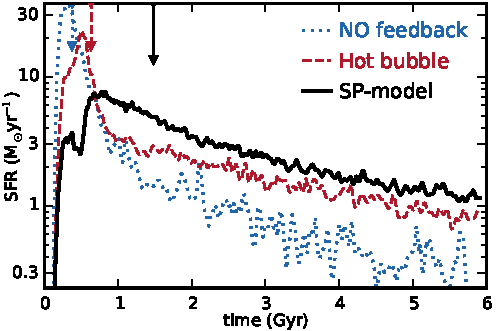
\includegraphics{sfr.pdf}
\caption{SFR as a function of time for our Milky Way-like isolated galaxy using three different SN feedback schemes: no energy feedback (NO feedback), purely thermal feedback to the five closest neighboring particles (Hot bubble), and the model SN energy feedback (SP-model), which transfers energy according to the physics of the SN phase (free expansion, Sedov-Taylor, or snowplow) in which each of the closest 10 neighboring particles lies. The vertical arrows indicate the age at which half the new galactic stellar mass has been assembled.}
\label{fig:SFR_isolated}
\end{figure}

\subsection{SFR and Galactic Characteristics}\label{subsec:res_sfr}
The most important effect of the SP-model feedback can be observed in the star formation history. Fig.~\ref{fig:SFR_isolated} shows the SFR for our isolated galaxy using all three SN feedback schemes considered. The SFR histories for the three feedback schemes differ more significantly during the early phases of the simulations, when the presence of feedback in kinetic form suppress SFR more efficiently. The SP-model feedback, which most effectively suppresses early star formation, has the highest rate of late-time star formation, as material partially ejected by a central ``fountain'' returns at later times to be incorporated in late forming stars. Under NO feedback, the current SFR is 0.23 M$_{\sun}$ yr$^{-1}$, compared to a value of 0.94 under Hot bubble feedback and 1.15 M$_{\sun}$ yr$^{-1}$ under SP-model feedback. The estimated value for the Milky Way is 0.68--1.45 M$_{\sun}$ yr$^{-1}$ \citep{Robitaille2010}. Had we allowed for growing torques from non-axisymmetric tidal forces, these effects would have been more pronounced \citep[see e.g.,][]{Brook14, Uebler14}.

The differences in star formation affect several other galactic characteristics. We therefore measure other important galactic quantities to better understand the impact of each feedback scheme. These measurements are shown in Table \ref{table:results}.

The strongly suppressed early star formation results in an overall younger stellar population, as indicated by the age at which half the new galactic stellar mass is assembled: 1.48 Gyr for SP-model feedback as opposed to 0.37 Gyr for NO feedback and 0.63 for Hot bubble feedback. These half ages are indicated by vertical arrows in Fig.~\ref{fig:SFR_isolated}.

The gas outflow rate (OFR) ---measured as the cumulative outflow rate of gas beyond $\pm$2 kpc from the plane of the disk over 6 Gyr--- suggests the existence of the strong fountain effect in SP-model: OFR is 0.01 M$_{\sun}$ yr$^{-1}$ under NO feedback, 0.37 M$_{\sun}$ yr$^{-1}$ under Hot bubble feedback, and 0.76 M$_{\sun}$ yr$^{-1}$ under SP-model feedback.

The mass loading factor $\eta$ ---measured as the OFR divided by the cumulative stellar mass produced over 6 Gyr--- is a very important metric for assessing the applicability of the models. For the NO feedback case it is 0.01, for the Hot bubble feedback case it is 0.36, and for the SP-model feedback case it is 0.72. \citet{Muratov15} found in their study of galactic winds using high-resolution cosmological simulations ---part of the \textsc{Fire} project--- that galaxies similar in size to our fiducial exhibit gusty outflows at high redshift ($z>1.0$) but then reach a moderate, steady SFR and subdued, weak outflows at low redshift ($z<0.5$). This translates into $\eta$ values close to 10 at high redshift and lower than 1 at low redshift\footnote{\citet{Muratov15} presents several different methods to measure $\eta$ for their simulated galaxies. Our method is most similar to their \textit{Cross T} method, albeit with different geometry in the threshold boundary to categorize the outflow.}.

The different SFR histories of the three feedback scenarios result in different stellar populations after 6 Gyr. Table~\ref{table:results} includes final halo and galactic characteristics. We define the virial radius to be $r_{200}$, the radius where the mean density drops below 200 times the critical density of the universe. We then define the galactic radius to be $r_{10}=0.1r_{200}$. The variations across the feedback scenarios of the virial mass and virial radius are small, as expected. The distinguishable impact of the SP-model lies in the age and mass distribution of the stellar population. 

The SP-model feedback generates a flatter disk structure in the inner 4 kpc of the galaxy than NO feedback and Hot bubble feedback. Fig.~\ref{fig:sigmacurves} shows surface density ---using dm/dr = 2$\pi r\Sigma(r)$--- at different galactic radii at the end of the simulations for all three SN feedback scenarios. Another indicator of the spread of stellar content is the effective radius $r_{\mathrm{eff}}$ ---the radius of a sphere circumscribing half of the stellar mass (vertical arrows in Fig.~\ref{fig:sigmacurves}). $r_{\mathrm{eff}}$ is larger under SP-model feedback NO feedback by a factor of 3.2, but it is smaller than under Hot bubble feedback by a factor of 0.8. We found no bar formation in our simulations.

\begin{table*}
\centering
%\begin{minipage}{145mm}
\caption{Simulations Results.}
\label{table:results}
\begin{threeparttable}
\begin{tabular}{@{\ \ }l@{\ \ \ }c@{ \ }c@{\ \ }c@{\ \ \ \ \ }c@{ \ }c@{ \ }c@{ \ }c@{\ \ }c@{\ \ \ \ \ }c@{ \ }c@{ \ }c@{ \ }c@{\ \ \ }c@{\ \ \ }c@{\ \ }}
\hline\hline
 & \multicolumn{2}{c}{Halo} & & \multicolumn{4}{c}{Galaxy} & & \multicolumn{6}{c}{Galactic Properties}\\
 & \multicolumn{2}{c}{\hrulefill} & & \multicolumn{4}{c}{\hrulefill} & & \multicolumn{6}{c}{\hrulefill} \\
SN Feedback &
$r_{\mathrm{200}}$ \tnote {a} &
$m_{\mathrm{200}}$ \tnote{b} & &
$r_{\mathrm{eff}}$ \tnote{c} &
$m_{\mathrm{10}}$ \tnote{d} &
$m_{\mathrm{*10}}$ \tnote{e} &
$m_{\mathrm{g10}}$ \tnote{f} & &
$f_{\mathrm{*}}$ \tnote{g} &
$L_X$ \tnote{h} &
$t_{1/2}$ \tnote{i} &
SFR \tnote{j} &
OFR \tnote{k} &
$\eta$ \tnote{l} \\

\multicolumn{1}{c}{Type} & (kpc) & & & (kpc) & & & & &(\%) & (erg s$^{-1}$)  & (Gyr) & \multicolumn{2}{c}{(M$_{\sun}$ yr$^{-1}$)} & \\[0.05 in]
\hline
\\[-1.5mm]
NO feedback & 162.14 & 94.89 & & 0.53 & 18.88 & 0.75 & 0.03 & & 4.7 & 5.1$\times 10^{38}$ & 0.37 & 0.23 & 0.01 & 0.01\\
Hot bubble  & 162.12 & 94.85 & & 2.09 & 18.93 & 0.61 & 0.16 & & 3.8 & 5.8$\times 10^{38}$ & 0.63 & 0.94 & 0.37 & 0.36\\
SP-model    & 162.09 & 94.80 & & 1.71 & 18.86 & 0.63 & 0.10 & & 3.9 & 9.9$\times 10^{38}$ & 1.48 & 1.15 & 0.76 & 0.72\\[2mm]
\hline\hline
\end{tabular}
\begin{tablenotes}
NOTE. -- All masses in units of $10^{10}$ M$_{\sun}$.
\item[a] virial radius; \item[b] virial mass; \item[c] radius of a sphere circumscribing half of the stellar mass; \item[d] galactic mass; \item[e] galactic stellar mass; \item[f] galactic gas mass; \item[g] percentage of galactic baryons converted into stars: $m_{*10}$/($m_{200}\times$ universal baryon fraction);  \item[h] current X-ray luminosity; \item[i] age at which half the new galactic stellar mass is assembled; \item[j] current star formation rate; \item[k] cumulative gas outflow rate from galactic disk over 6 Gyr; \item[l] mass loading factor: cumulative gas outflow from galactic disk divided by the cumulative stellar mass produced over 6 Gyr.
\end{tablenotes}
\end{threeparttable}
%\end{minipage}
\end{table*}


\begin{figure}
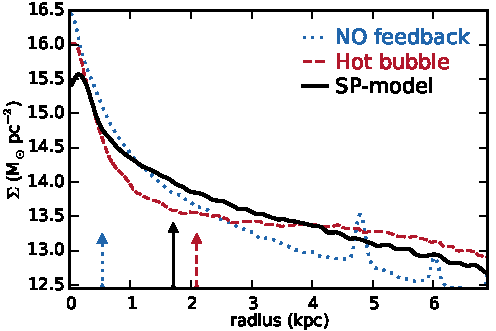
\includegraphics{sigmacurves.pdf}
\caption{Current surface density curves for our simulated galaxy using three different SN feedback schemes. The vertical arrows indicate the effective radius $r_{\mathrm{eff}}$ of a sphere circumscribing half of the new stellar mass.}
\label{fig:sigmacurves}
\end{figure}

Fig.~\ref{fig:rot_isolated} shows the theoretical circular velocities $v_{\mathrm{c}}=\sqrt{Gm(r)/r}$ of each galactic component for the initial conditions (IC) (top panel), the NO feedback scenario (upper middle panel), the Hot bubble feedback scenario (lower middle panel), and the SP-model feedback scenario (bottom panel). The SP-model feedback creates a significantly flatter rotational curve for the new stellar component (black solid line) compared to NO feedback and Hot bubble feedback. Under the SP-model feedback, the mean $v_{\mathrm{c}}$ for gas and star particles within $r_{10}$  at the end of the simulation are 24 km s$^{-1}$ and 99 km s$^{-1}$, respectively, compared to 55 km s$^{-1}$ and 69 km s$^{-1}$ in the initial conditions. Interestingly, the old bulge stellar component (orange dashed line) ends up with a significantly flatter rotational curve under the NO feedback and Hot bubble scenarios. We suspect this is caused by a transfer of angular momentum from the bulge star particles to the new star particles, as a significant portion of the star formation occurs near the galactic bulge. The latter is a direct consequence of the absence of energy transfer in the NO feedback scenario and lack of kinetic energy feedback in the Hot bubble scenario, which would otherwise help push out hot gas from star forming regions.

\begin{figure}
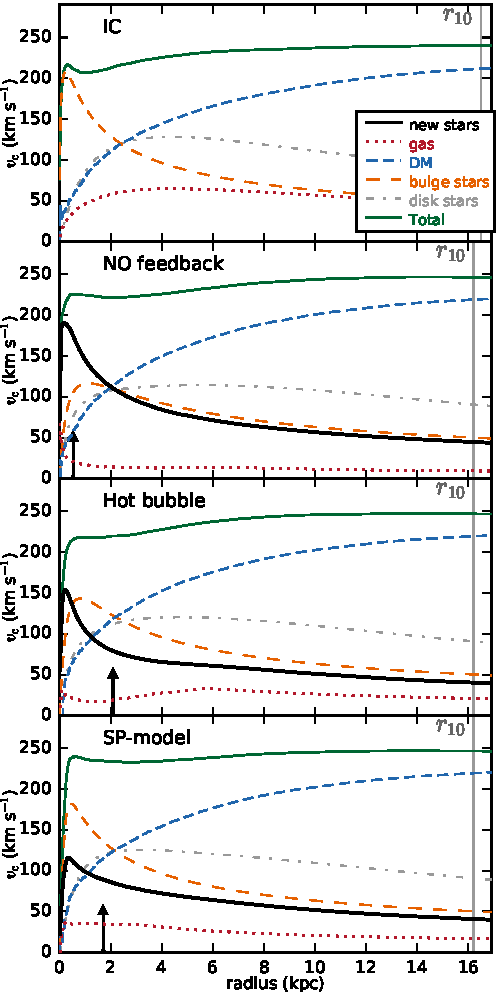
\includegraphics{rotcurves.pdf}
\caption{Rotational curves for each galactic component for the initial conditions (IC) (upper panel), at end of simulation using a NO feedback scheme (upper middle panel), using a Hot bubble feedback scheme (lower middle panel), and using the SP-model scheme (bottom panel). The galactic radius $r_{10}=0.1 r_{200}$ is indicated with a vertical grey line. The vertical arrows indicate the effective radius $r_{\mathrm{eff}}$ of a sphere circumscribing half of the new stellar mass.}
\label{fig:rot_isolated}
\end{figure}

To compare how stellar populations assemble in the galaxy, Fig.~\ref{fig:masses_isolated} shows a history of stellar (top panel) and gas (bottom panel) masses within the galactic radius $r_{10}$ for all three feedback scenarios. The vertical arrows indicate the time when the galaxy has assembled half of its new stellar mass. In the NO feedback scenario (dotted line), the new stellar content of the galaxy accumulates quickly, whereas any form of energy feedback (Hot bubble or SP-model) hinders this process significantly. Consequently, gas is very quickly depleted under NO feedback, as seen in the bottom panel. Both the Hot bubble and SP-model feedback schemes allow more gas to remain by either heating it or kicking some of it out of the galaxy early on and allowing it to later rain back into the disk. After 6 Gyr the gas-to-stellar-mass ratio is significantly higher when the SP-model is in place (0.16) compared to NO feedback (0.04).

\begin{figure}
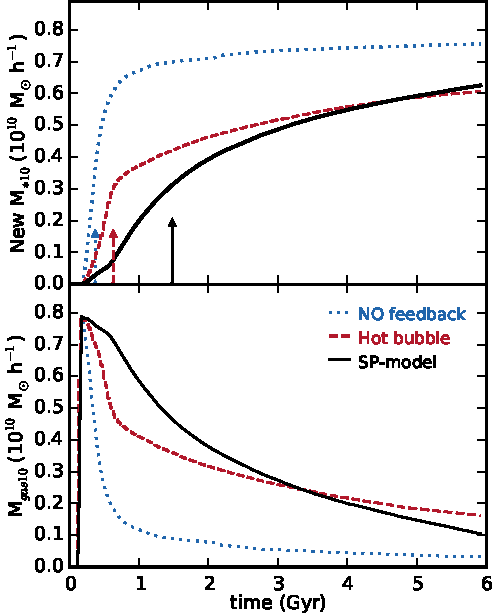
\includegraphics{galactic_masses.pdf}
\caption{New stellar mass (top panel) and gas mass (bottom panel) within the galactic radius $r_{10}=0.1 r_{200}$ as a function of time for three different SN feedback schemes. The vertical arrows indicate the time when the galaxy assembled half of its new stellar mass.}
\label{fig:masses_isolated}
\end{figure}

\subsection{Energy Transfer}\label{subsec:res_Etransfer}
Figs.~\ref{fig:diag_isolated_Etransferred}--\ref{fig:diag_isolated_K-Th_sp} present a breakdown of the energy transferred in type II SN events. They help to illustrate in more detail how the SP-model feedback distributes energy to the surrounding medium.

According to the description of the SP-model feedback in Sec.~\ref{subsubsec:phases}, some SN energy is radiatively lost during the SP phase (outside $r_{\mathrm{cool}}$), whereas no energy is lost during the FE and ST phases. Therefore, the total amount of energy transferred to gas particles is not always equal to the original SN energy of the ejecta. Fig.~\ref{fig:diag_isolated_Etransferred} shows a normalized histogram of the fraction of type II SN energy released by a star particle that is actually transferred to neighboring gas particles. In $\approx$40\% of the cases, the fraction of the original SN energy transferred is 80\% or greater, either because neighboring gas particles are in FE or ST phase, where no SN energy is lost, or because they are within the SP phase but not too far from the ST--SP transition radius $r_{\mathrm{cool}}$, thus allowing only a small fraction of the original SN ejecta energy to be lost in cooling. By construct, most of the energy in the FE phase, ST phase, and SP phase near $r_{\mathrm{cool}}$ is in thermal form. On the other hand, $\approx$10\% of the cases resulted in an energy transfer less than 20\% of the original SN energy transferred to neighboring gas particles. This is a consequence of gas particles being far into the SP phase, i.e., well outside the ST--SP transition radius $r_{\mathrm{cool}}$, where a significant portion of the original SN energy is lost via radiative cooling. Most of the energy in the SP phase far from $r_{\mathrm{cool}}$ is in kinetic form, as the thermal portion of the remaining energy dissipates more quickly than the kinetic portion (see Eqs.~\ref{E_Th} and \ref{E_K}). Thus, for the cases where most of the original SN energy is dissipated, almost all of the energy transferred is in kinetic form.

\begin{figure}
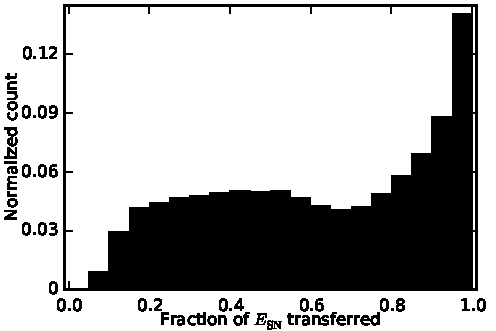
\includegraphics{SN_frac_transferred.pdf}
\caption{Normalized histogram of the fraction of type II SN feedback energy transferred to neighboring gas particles.}
\label{fig:diag_isolated_Etransferred}
\end{figure}

Fig.~\ref{fig:diag_isolated_PhasesE} illustrates the fraction of energy transferred at the different SNR phases as a function of time. Most SN energy is transferred to gas particles lying within the ST phase (red region) for three main reasons: first, no energy loss occurs during the ST phase; second, neighboring gas particles in the ST phase have larger SPH kernel weights than those in the SP phase; and third, $r_{\mathrm{cool}}$ increases as ISM densities drop, the latter driven by SN feedback. Also, not many gas particles are found in the FE phase, which is subject to simulation resolution. Finally, Fig.~\ref{fig:diag_isolated_PhasesE} shows that during the first $\approx$1 Gyr of the simulation the majority of the energy is transferred to gas particles in the SP phase. According to Eq.~\ref{STradius}, this indicates that initial high $n_0$ values and low $f_{\mathrm{hot}}$ values --- and thus, small $r_{\mathrm{cool}}$--- must have shifted to lower $n_0$ and higher $f_{\mathrm{hot}}$ values rather rapidly, which in turn increased $r_{\mathrm{cool}}$, such that after $\approx$1 Gyr the energy transferred in the SP phase decreased from almost 100 to $\approx$50\% of the total.

\begin{figure}
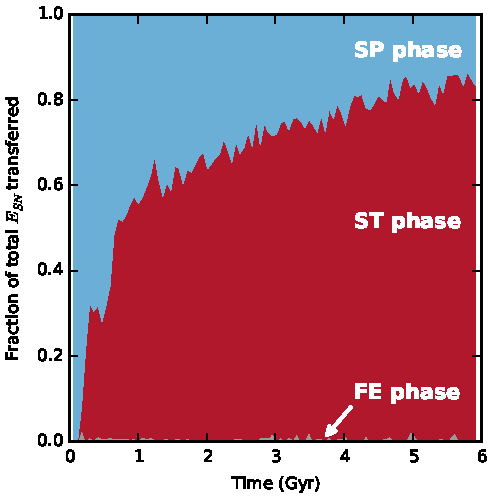
\includegraphics{SN_phases_energy.pdf}
\caption{Fraction of total transferred type II SN energy at each SNR phase as a function of time when the SP-model energy feedback scheme is implemented on our Milky Way-like isolated galaxy.}
\label{fig:diag_isolated_PhasesE}
\end{figure}

Fig.~\ref{fig:diag_isolated_K-Th_sp} shows the fraction of total energy transferred in the form of kinetic and thermal energy as a function of time. During the first $\approx$1 Gyr, the time during which most energy transfer occurs in the SP phase, the majority of energy transferred is kinetic. This drives early strong winds out of the galactic disk, which help suppress early star formation significantly. Furthermore, the fraction of energy transferred never falls below 30\% (gray dashed line) for 6 Gyr, which illustrates the effect of increasing kinetic energy transfer when the SP phase is included in SN feedback. 

\begin{figure}
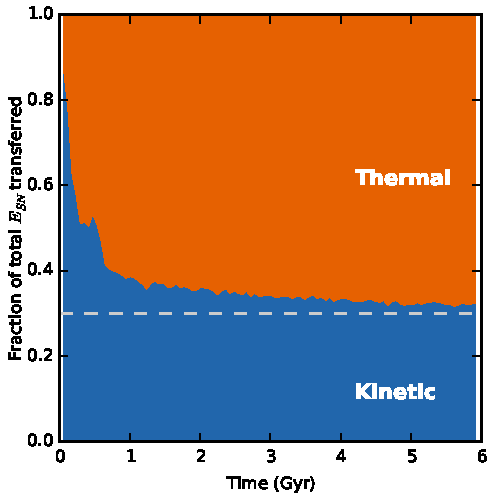
\includegraphics{SN_energy.pdf}
\caption{Fraction of total transferred type II SN energy as either kinetic (blue) or thermal (orange) form when the SP-model energy feedback scheme is implemented on our Milky Way-like isolated galaxy. The gray dashed line indicates the limit where 30\% of energy is transferred in kinetic form, which is the case during the ST phase of the SP-model feedback scheme.}
\label{fig:diag_isolated_K-Th_sp}
\end{figure}

Lastly, we note that in the extreme case of a large hot volume fraction $f_{\mathrm{hot}}$, the amount of transferred thermal and kinetic energy approximates the type of feedback present in the ST phase, not only because the ST--SP transition radius $r_{\mathrm{cool}}$ increases in size (Eq.~\ref{STradius}), but also because the radial factor in Eqs.~\ref{E_Th} and \ref{E_K} approaches unity. We tested a simulated galaxy using exclusively ST feedback on all neighboring gas particles and found that the results were very similar to the results using the SP-model feedback.

\subsection{X-rays}\label{subsec:res_Xrays}
As noted by \citet{Boroson11}, a correlation is expected between the hot gas content and gravitational potential of the galaxy. These authors measured X-ray emission by hot and diffuse gas in galactic halos in the range 0.3--8 keV as proxy for the hot gas content, and central velocity dispersion $\sigma$ as proxy for the gravitational potential, on a sample of 30 early-type galaxies observed with \textit{Chandra}.

To verify this correlation in our simulated galaxies, we estimate the total galactic X-ray luminosity $L_{\mathrm{X}}$ using an emissivity prescription, described in \citet{Choi14}, that includes bremsstrahlung radiation and line emissions of all tracked species within the 0.3--8 keV band produced by hot ($T \ge 10^6$ K) and diffuse ($\rho \le 2.14\times 10^{-25}$ g cm$^{-3}$) gas halo particles. We then measure circular velocity $\langle v_c \rangle$ as the mass-weighted mean rotational velocity for star particles within the galactic disk $r_{10}$. We compare our $\langle v_c \rangle$ values against the measured $\sigma$ in \citet{Boroson11}. We convert their $\sigma$ values into $\langle v_c \rangle$ using $\langle v_c \rangle^2$ $\approx$ $2\sigma^2$. We find that, given the $\langle v_c \rangle$ values of our simulated galaxies, $L_{\mathrm{X}}$ falls within the observed locus defined in \citet{Boroson11}. Fig.~\ref{fig:Lx_isolated} shows $L_{\mathrm{X}}$ versus $\langle v_c \rangle$ of our isolated galaxy for all three feedback scenarios. Only small $L_{\mathrm{X}}$ differences are seen between the three models, with the SP-model feedback resulting in a $L_{\mathrm{X}}$ value higher than the Hot bubble feedback by a factor of 2. This is probably caused by the large fraction of kinetic energy transferred to the disk gas near SN events at early epochs (see Fig.~\ref{fig:diag_isolated_K-Th_sp}), which pushes it farther into the galaxy halo.

Also, if we consider the mass--$L_{\mathrm{X}}$ relation found by \citet{Anderson15} (see bottom panel of their figure 5) on a large sample of bright galaxies from the Sloan Digital Sky Survey (SDSS), we find that given the current total stellar mass content of our simulated galaxy ($\sim$5$\times 10^{10} M_{\sun}$), its halo $L_{\mathrm{X}}$ falls within the trend observed in the range 10$^{10}-10^{12} M_{\sun}$.

\begin{figure}
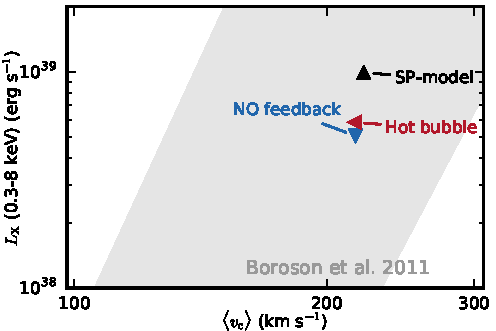
\includegraphics{Lx_sigma.pdf}
\caption{X-ray luminosity $L_{\mathrm{X}}$ of our Milky Way-like isolated galaxy versus circular velocity $\langle v_c \rangle$ for three different feedback schemes. We calculate $\langle v_c \rangle$ as the mass-weighted mean rotational velocity for star particles within the galactic radius $r_{10}$. To calculate $L_{\mathrm{X}}$ we use an emissivity prescription that includes bremsstrahlung radiation and line emissions of all tracked species within the 0.3--8 keV band produced by hot ($T \ge 10^6$ K) and diffuse ($\rho \le 2.14\times 10^{-25}$ g cm$^{-3}$) gas halo particles. The observed relation (in light gray) is from \citet{Boroson11}. We translate their measurements of central velocity dispersion $\sigma$ into $\langle v_c \rangle$ using $\langle v_c \rangle^2 \approx 2\sigma^2$.}
\label{fig:Lx_isolated}
\end{figure}

\subsection{Metallicity}\label{subsec:res_metallicity}
Since the different SN feedback mechanisms affect differently the rate and time of star formation, they also affect the final metal content of both gas and star particles in the galaxy. As we described in Sec.~\ref{subsec:sfr}, ejected material from type Ia and II SNe, as well as from AGB and young massive stellar winds, is composed of several metal species in addition to hydrogen and helium.

Under NO feedback, the current median metallicity of the new stellar mass log(Z/Z$_{\sun}$) of our simulated galaxy is 0.11$^{+0.35}_{-0.49}$ (upper and lower bounds indicate the 16th and 84th percentiles); under Hot bubble feedback, it is 0.26$^{+0.33}_{-0.60}$; and under the SP-model feedback, it is 0.34$^{+0.29}_{-0.62}$. The SP-model feedback increases stellar metallicity by a factor of 1.7 compared to NO feedback, and by a factor of 1.2 compared to Hot bubble feedback.

These values, however, do not account for the fact that we do not track metallicity for primordial disk and bulge stars in our galaxy. Therefore, to determine the median metallicity for the entire stellar content, we estimate the median metallicity of this primordial stellar mass using the empirical stellar mass--metallicity relation in \citet{Gallazzi2005}. These authors calculated the median and 16$^{th}$ and 84$^{th}$ percentiles of the distributions in stellar metallicity as a function of stellar mass for a sample of high-quality SDSS spectra of galaxies that includes both early- and late-type galaxies. Given the total mass of the primordial bulge and disk stars in our galaxy (5.3$\times 10^{10}$ M$_{\sun}$), we find that their metallicity ought to be log(Z/Z$_{\sun}$) = $0.04^{+0.22}_{-0.24}$ according to this relation. Using this value, the mass-weighted stellar metallicity for the entire stellar mass content of our galaxy under SP-model feedback is $0.07^{+0.30}_{-0.35}$. This value is statistically similar to the one obtained using the \citet{Gallazzi2005} relation for a galaxy with the same total stellar content as ours. We consider this result only as guidance, since in our isolated galaxy scenario we do not account for external galactic events ---such as mergers or infall of primordial cosmological gas--- that could alter the metal content of galaxies.

Fig.~\ref{fig:Metals} shows the stellar radial metallicity distribution in the galaxy under NO feedback (blue dotted line), Hot bubble feedback (red dashed line), and SP-model feedback (solid black line). A linear regression analysis in the inner part of the disk ($r/r_{\mathrm{eff}}<5$) indicates that the stellar metallicity gradient becomes shallower in the SP-model feedback case ($-0.05\pm0.01$) compared to the NO feedback case ($-0.10\pm0.01$) and Hot bubble case ($-0.13\pm0.01$). \citet{Sanchez-Blazquez2014} found for their sample of 62 spiral galaxies from the CALIFA survey a mean slope of $-0.087\pm0.008$. These authors did not specify zero points in their linear fits, and so we used the zero point from our fit to over-plot their result (gray line) in Fig.~\ref{fig:Metals}.

The median galactic gas metallicity increases from 12 + log(O/H) = 8.91$^{+0.14}_{-0.04}$ under NO feedback, to 9.53$\pm0.01$ under Hot bubble feedback, to 9.61$\pm0.02$ under the SP-model feedback. \citet{Tremonti2004} found a median gas metallicity for galaxies similar in stellar content to ours of 12 + log(O/H) = $8.90^{+0.11}_{-0.10}$ in their sample of SDSS galaxies at $0.005 < z < 0.25$. Similarly, \citet{Andrews2013} measure 12 + log(O/H) = 8.75$\pm0.02$ for galaxies similar in stellar content to ours.

The higher-than expected gas metallicity in our simulated galaxy with SP-model feedback may also reflect the inclusion of galaxies at higher redshifts and of early-type galaxies in these empirical samples. Nevertheless, the trend of higher gas metallicity with the SP-model suggests that more metal content is reaching more gas in the disk of the galaxy. The gradient of gas metallicity decreases from $-0.09\pm0.01$ (NO feedback) to $\approx$-0.01 (SP-model feedback). \citet{Sanchez2014} found for their sample of 306 galaxies from the CALIFA survey a characteristic slope of $-0.10\pm0.09$ (with a zero-point of 12+log(O/H) $=8.73\pm0.16$ between 0.3 and 2 $r_{\mathrm{eff}}$).

There is an important effect that may also explain our higher than expected gas metal content. In our own Milky Way galaxy the deuterium abundance is close to 80\% of the primordial abundance, indicating that inflowing pristine and metal-free gas makes up a non negligible fraction of the observed local ISM. Thus, if we made allowance for cosmological infall of gas in our simulations, the metal abundance in our galaxies would be significantly lower.

\begin{figure}
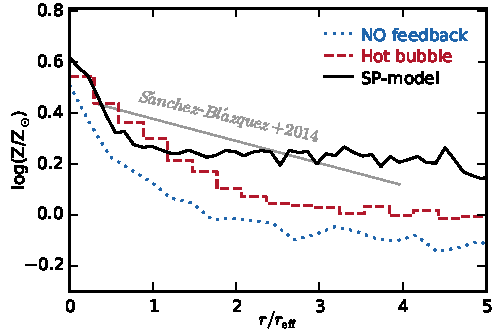
\includegraphics{metallicity_gradient.pdf}
\caption{Radial distribution of the stellar metallicity content in the galaxy under three different SN feedback schemes. Results from \citet{Sanchez-Blazquez2014} on samples of galaxies from the CALIFA survey are indicated with a gray line. We used the zero point from our own linear regression analysis to indicate their result.}
\label{fig:Metals}
\end{figure}

\subsection{Sensitivity to Ejecta Velocity Parameter}\label{vejecta}
To explore the sensitivity of the SP-model scheme to the ejecta velocity parameter $v_{\mathrm{ej}}$, we re-ran our simulations with the SP-model feedback changing $v_{\mathrm{ej}}$ from our fiducial value of 4500 km s$^{-1}$ to 3000, 6000, and 7500 km s$^{-1}$. We find that the baryon conversion efficiency $f_{*}$ --- defined as $m_{*10}/(m_{200}\times f_{\mathrm{bar}})$, where $f_{\mathrm{bar}}\approx 0.17$--- decreases as $v_{\mathrm{ej}}$ increases: $f_{*}$ goes from 0.042 to 0.032 and 0.024 for $v_{\mathrm{ej}}=3000$, 6000, and 7500 km s$^{-1}$, respectively. Under the NO feedback scenario ---which serves as a proxy for $v_{\mathrm{ej}}=0$ km s$^{-1}$, $f_{*}= 0.047$. The mass loading parameter $\eta$ increases with increasing $v_{\mathrm{ej}}$, from 0.39 to 0.95 and 1.72 for $v_{\mathrm{ej}}=$ 3000, 6000, and 7500 km s$^{-1}$, respectively. Under the NO feedback scenario, $\eta=0.01$. This highlights the sensitivity of the fountain effect to the parameter $v_{\mathrm{ej}}$, particularly when $v_{\mathrm{ej}}$ has a value greater than our fiducial. Lastly, the galactic halo is significantly affected as we increase $v_{\mathrm{ej}}$ beyond our fiducial value: the galactic halo $L_{\mathrm{X}}$ increases by a factor of 11 when we increase $v_{\mathrm{ej}}$ from 4500 to 6000 km s$^{-1}$, and by a factor of 19 when we increase it to 7500 km s$^{-1}$.

There appears to be an energy feedback threshold ---dependent on $v_{\mathrm{ej}}$ according to Eq.~\ref{E_SN}--- beyond which a nascent galaxy at high redshift is strongly compromised by SNR winds. Clearly, this threshold is the point at which the SN ejecta velocity starts reaching the escape velocity of the system. The ejecta velocity would thus set the limit of the halo mass below which the resulting stellar mass would be very small. The peak ratio of stellar to DM mass \citep{Guo10} occurs at stellar mass of 2.2$\times 10^{10}$ M$_{\sun}$, with a strongly observed decline for lower mass systems, which have lower escape velocities.

\subsection{Comparison of Results at Different Resolution Levels}\label{resolutions}
To test convergence of results at different numerical resolution levels, we ran low and high resolution simulations in addition to our fiducial resolution simulation using the SP-model feedback with 10 times lower and 10 times higher mass resolution, respectively. Table~\ref{table:resolutions} describes the SPH particle parameters for the low and high resolution levels.

\begin{table}
\centering
\caption{Comparison of SPH Particles Parameters at Different Resolution Levels.}
\label{table:resolutions}
\begin{threeparttable}
\newcolumntype{d}{D{.}{.}{-1}}
\begin{tabular}{rcdcdcc}
\hline\hline
 & \multicolumn{3}{c}{Low Res} & \multicolumn{3}{c}{High Res} \\
 & \multicolumn{3}{c}{\hrulefill} & \multicolumn{3}{c}{\hrulefill} \\
\multicolumn{1}{c}{Par.} & \multicolumn{1}{c}{N\tnote{a}} & \multicolumn{1}{c}{Mass\tnote{b}} & \multicolumn{1}{c}{$\epsilon$\tnote{c}} & \multicolumn{1}{c}{N\tnote{a}} & \multicolumn{1}{c}{Mass\tnote{b}} & \multicolumn{1}{c}{$\epsilon$\tnote{c}} \\
\multicolumn{1}{c}{Type} & \multicolumn{1}{c}{(10$^4$)} & \multicolumn{1}{c}{(10$^5$)} & \multicolumn{1}{c}{(kpc)} & \multicolumn{1}{c}{(10$^4$)} & \multicolumn{1}{c}{(10$^5$)} & \multicolumn{1}{c}{(kpc)}\\[0.05 in]
\hline
\multicolumn{1}{l}{Gas}   & & & & & & \\
\textit{Halo}  & 0.18 & 13.0 & 0.092 & 17.59 & 0.13 & 0.02 \\
\textit{Disk}  & 0.94 & 13.0 & 0.092 & 94.46 & 0.13 & 0.02 \\
\multicolumn{1}{l}{Stars} & & & & & & \\
\textit{Disk}  & 2.40 & 13.0 & 0.092 & 240.0 & 0.13 & 0.02 \\
\textit{Bulge} & 0.75 & 13.0 & 0.092 & 75.0  & 0.13 & 0.02 \\
\multicolumn{1}{l}{DM} & 3.00 & 446.6 & 0.460 & 300.0 & 4.47 & 0.10 \\[0.05 in]
\hline\hline
\end{tabular}
\begin{tablenotes}
\item[a] Number of particles;
\item[b] per particle, in units of M$_{\sun}$;
\item[c] gravitational softening length.
\end{tablenotes}
\end{threeparttable}
\end{table}

Fig.~\ref{fig:SFR_res} compares the SFR amongst the three resolution levels tested. We find that to first order, SFR converges with resolution, with the high-resolution case having slightly more spikes of star formation at very early epochs than the other two cases. Overall, however, the high resolution case results in higher stellar and gas content in the galaxy: gas-to-star mass ratio goes from 0.3 in the low resolution case to 0.6 in the high resolution case. The high resolution case also results in younger stellar content: $t_{1/2}$ increases from 1.4 Gyr in the low resolution case to 1.8 Gyr in the high resolution case.

Similarly, to first order, surface density converges with resolution. However, higher resolution results in a slightly more spread-out, flatter stellar content. Fig.~\ref{fig:sigmacurves_res} shows the surface density curves for the three resolution cases becoming slightly flatter with higher resolution. Also, $r_{\mathrm{eff}}$ (vertical lines in Fig.~\ref{fig:sigmacurves_res}) increases from 1.3 kpc in the low resolution case to 2.1 kpc in the high resolution case. Lastly, the mass loading factor $\eta$ increases to 5.4 in the low resolution case, and to 1.7 in the high resolution case. Several parameter values are compared in Table~\ref{table:results_res} for the three resolution levels.

\begin{figure}
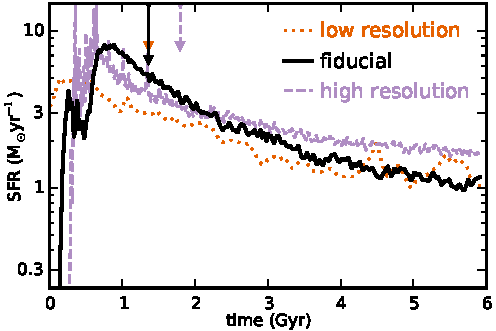
\includegraphics{sfr_res.pdf}
\caption{SFR as a function of time for our Milky Way-like isolated galaxy using the model SN energy feedback SP-model scheme at low resolution (dotted orange line), our fiducial mid resolution (solid black line), and high resolution (dashed purple line) levels. The vertical arrows indicate the age at which half the new galactic stellar mass has been assembled.}
\label{fig:SFR_res}
\end{figure}

\begin{figure}
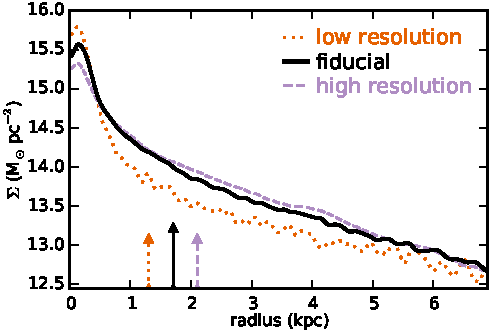
\includegraphics{sigmacurves_res.pdf}
\caption{Current surface density curves for our simulated galaxy using the model SN energy feedback SP-model scheme at low, mid (fiducial), and high resolution levels. The vertical arrows indicate the effective radius $r_{\mathrm{eff}}$ of a sphere circumscribing half of the new stellar mass.}
\label{fig:sigmacurves_res}
\end{figure}

\begin{table*}
\centering
\caption{Simulations Results at Different Resolution Levels Using the SP-model Feedback.}
\label{table:results_res}
\begin{threeparttable}
\begin{tabular}{@{\ \ }l@{\ \ \ }c@{ \ }c@{\ \ }c@{\ \ \ \ \ }c@{ \ }c@{ \ }c@{ \ }c@{\ \ }c@{\ \ \ \ \ }c@{ \ }c@{ \ }c@{\ \ \ }c@{\ \ \ }c@{\ \ }}
\hline\hline
 & \multicolumn{2}{c}{Halo} & & \multicolumn{4}{c}{Galaxy} & & \multicolumn{5}{c}{Galactic Properties}\\
 & \multicolumn{2}{c}{\hrulefill} & & \multicolumn{4}{c}{\hrulefill} & & \multicolumn{5}{c}{\hrulefill} \\
Resolution &
$r_{\mathrm{200}}$ \tnote {a} &
$m_{\mathrm{200}}$ \tnote{b} & &
$r_{\mathrm{eff}}$ \tnote{c} &
$m_{\mathrm{10}}$ \tnote{d} &
$m_{\mathrm{*10}}$ \tnote{e} &
$m_{\mathrm{g10}}$ \tnote{f} & &
$f_{\mathrm{*}}$ \tnote{g} &
$t_{1/2}$ \tnote{i} &
SFR \tnote{j} &
OFR \tnote{k} &
$\eta$ \tnote{l} \\

\multicolumn{1}{c}{Level} & (kpc) & & & (kpc) & & & & & (\%) & (Gyr) & \multicolumn{2}{c}{(M$_{\sun}$ yr$^{-1}$)} & \\[0.05 in]
\hline
\\[-1.5mm]
Low Res  & 161.53 & 94.13 & & 1.30 & 18.93 & 0.48 & 0.15 & & 3.0 & 1.36 & 1.00 & 4.29 & 5.39\\
Fiducial & 162.09 & 94.80 & & 1.71 & 18.86 & 0.63 & 0.10 & & 3.9 & 1.48 & 1.15 & 0.76 & 0.72\\
High Res & 162.80 & 96.42 & & 2.10 & 19.45 & 0.64 & 0.40 & & 3.9 & 1.79 & 1.62 & 1.78 & 1.67\\[0.05 in]
\hline\hline
\end{tabular}
\begin{tablenotes}
NOTE. -- All masses in units of $10^{10}$ M$_{\sun}$. Notes (a) to (l) are defined in Table~\ref{table:results}.
\end{tablenotes}
\end{threeparttable}
\end{table*}
 
\section{Conclusions}\label{sec:conclusions}
We implement a physically motivated stellar feedback model, including winds from young and old stars, heating from young massive stars, and a SN energy feedback formulation (``SP-model'') that allows for cooling of the original SN ejecta, with the thermal portion dissipating away more quickly than the kinetic portion. The SP-model mimics the known physics that takes place during all phase of SNRs ---free expansion (FE) phase, Sedov-Taylor (ST) phase, and snowplow (SP) phase--- as revealed by both observations and high spatial resolution simulations. It also allows for the important effects of significantly enhanced SN remnant propagation in a multiphase medium. We implement this on an isolated Milky Way-type galaxy with a hot gas halo assembled following the methods in \citet{Springel05a} using the improved TreeSPH code SPHGal \citep{Hu14}, and we evolve it for 6 Gyr.

We also implement wind feedback from both young massive stars and older AGB stars by conserving momentum of the ejected material. For the former, we approximate the ejected material to be commensurate both in mass and velocity with that of type II SN explosions, except that we spread it evenly during the first 3 Myr of the life of the star particle. For the latter, we use mass yield prescriptions found in the literature and an ejecta velocity of 10 km s$^{-1}$, and we implement it throughout several Gyr following type II SN events.

We also implement two mechanisms that limit cooling of the ISM gas, one produced by the Str\"omgren sphere heating surrounding young massive stars, and the other one produced by the radiative recombination processes in dense H\textsc{ii} regions.

In our simulations the SP-model feedback addresses the sub-resolution physics problem in low resolution SPH simulations in which particle distances are barely resolved at the level necessary to allow for FE feedback, the type that many galaxy simulations include. By formulating a type of SN feedback that occurs mainly during the later stages of an SNR, namely ST and SP phases, the SP-model feedback allows for a more accurate representation of the physics involving SN energy feedback.

Given that both ST and SP phases allow for $\geq$ 30\% of the SN ejecta energy to be transferred in kinetic form, and that during SP phase the thermal energy fraction dissipates more quickly with distance than the kinetic fraction, gas particles surrounding SN events receive much stronger momentum kicks while in the ST and SP phases compared to the FE phase, in which feedback is driven by ejecta momentum conservation only. The result of implementing the SP-model feedback is a much flatter SFR history compared to a purely thermal SN feedback (here called Hot bubble feedback) and to having no energy feedback at all. As a consequence, the half age of the formed stars under the SP-model feedback is 4 times later than under no feedback and 2.3 times later than under Hot bubble feedback. The final SFR of the galaxy increases by a factor of 1.2 ---to 1.15 M$_{\sun}$ yr$^{-1}$--- as we go from Hot bubble feedback to the SP-model feedback.

The assembly of the galactic stellar content is more spread out in time in a galaxy with SP-model feedback, as much of the gas kicked out by the SNRs at early times eventually falls back to the galaxy, the so-called galactic ``fountain'' effect, where it cools off and is subject to star formation. The SP-model feedback results in a gas outflow rate from the galaxy of 0.76 M$_{\sun}$ yr$^{-1}$, compared to 0.01 M$_{\sun}$ yr$^{-1}$ under no stellar feedback and 0.37 under Hot bubble feedback. This fountain created by the SP-model feedback helps alleviate the issue of over clustering of stellar content at the galactic center, resulting in flatter rotational curves for the stellar component of the galaxy, flatter surface density curves for the galactic disk, and an overall larger galactic size, with the effective radius increasing by a factor of 3.2 as we go from having no stellar feedback to the SP-model feedback. Furthermore, the SP-model feedback results in a mass loading parameter $\eta$ of 0.72, versus 0.36 under Hot bubble feedback and 0.01 under no feedback.

The integrated stellar metallicity of our galaxy increases by a factor of 1.7 [measured as log(Z/Z$_{\sun}$)], and gas metallicity, by a factor of 5.0 [measured as 12+log(O/H)] as we go from having no stellar feedback to the SP-model feedback. The stellar metallicity disk gradients turn shallower under SP-model feedback ($-0.06$) compared to Hot bubble feedback ($-0.13$).

Given that the parameters of the SP-model ---phase transition radii, energy and mass input--- all scale with the SPH particle masses, our model is only weakly dependent on simulation resolution. The SP-model, however, does not completely address the problem of SN events occurring in overly dense regions in these simulations, which are a pure artificial construct of the limitation in spatial resolution. The unphysical result is SN events occurring in very dense regions that would otherwise be hollowed out by previous SN explosions.

In fact, nature has provided the solution: spatially displacing a significant fraction of type II SN events from their original location would lead to SN energy being released in less dense regions of the ISM. Many OB stars are ``runaways'' ---massive stars with high velocity dispersions resulting from the acceleration given by their SN-exploding, close binary companions. As \citet{Li15} points out, close to 40\% of type II SN explosions are from runaway OB stars, with their high velocity dispersions allowing them to travel up to 100--500 pc from their place of origin. A significant fraction of Type II SN events would, therefore, occur in low-density environments such as above the star forming disk or in inter-spiral arm regions.   

\section*{ACKNOWLEDGMENTS}
We thank Miao Li for valuable comments and feedback and Michaela Hirschmann for her insights into observed galactic metallicities. The simulations used here were run on Columbia University's Yeti cluster and the Max Planck Computing and Data Facility.

\bibliography{references}

\appendix

\section{Description of the SP-model for SPH Simulations.}\label{appendix}
As described in Sec.~\ref{subsubsec:implementation}, the SP-model feedback formulation states that a neighboring gas particle \textit{j} can receive energy from the SN event in one of three different ways, depending on its distance to the star particle relative to the phase transition radii $r_{\mathrm{ST}}$ and $r_{\mathrm{cool}}$ (Eqs. \ref{FEradius} and \ref{STradius}).

The FE-ST transition radius $r_{\mathrm{ST}}$ depends on the density of the medium, and the ST-SP transition radius $r_{\mathrm{cool}}$ depends on both the density and the temperature of the medium, the latter via the dependency of the hot volume fraction $f_{\mathrm{hot}}$ on the gas temperature (Eq.~\ref{fhot}). To allow for sharp density and temperature gradients around the star particle, we calculate both $r_{\mathrm{ST}}$ and $r_{\mathrm{cool}}$ for each of the closest 10 neighboring gas particles using the gas particle density $\rho_j$ and temperature $T_j$. The total amount of energy assigned to particle \textit{j} from the SN event is
\begin{equation}\label{delE}
\Delta E_j = w_j\ E_{\mathrm{SN}},
\end{equation}
where $w_j$ is the SPH kernel weight assigned to particle \textit{j} (in our simulations we use the Wendland $C^4$ kernel). The transfer of this energy affects three basic quantities in particle \textit{j}: its mass, its velocity, and its entropy (via addition of thermal energy). For the mass, one simply adds to the mass of particle \textit{j}, $M_j$, the value $\Delta m_j = w_j\ M_{ej}$. How the other two quantities change varies from one SNR phase to the other.

\subsection{FE Phase}
If particle \textit{j} is in the FE phase, then momentum conservation applies. The velocity vector to add to particle \textit{j}, assuming a perfectly non-elastic collision with the ejecta, is
\begin{equation}\label{FE_vadd}
\boldsymbol{\Delta v_{\mathrm{FE}}} = \frac{\epsilon}{1+\epsilon}\ (\boldsymbol{v_{\mathrm{ej}}} -\boldsymbol{v_j}),
\end{equation}
where $\epsilon=\Delta m_j/M_j$, $\boldsymbol{v_{\mathrm{ej}}}$ is the ejecta velocity and $\boldsymbol{v_j}$ is the velocity of particle \textit{j} before the collision. All three velocities are with respect to the star particle's rest frame. $\boldsymbol{\Delta v_{\mathrm{FE}}}$ is added to $\boldsymbol{v_j}$ radially away from the star particle.

To conserve energy, one must increase the thermal energy of particle \textit{j} by
\begin{equation}\label{FE_Ethadd}
\Delta E_{\mathrm{Th,FE}} = \frac{1}{2}\ \mu \ (\boldsymbol{v_{\mathrm{ej}}} -\boldsymbol{v_j})^2,
\end{equation}
where $\mu=\Delta m_j\ M_j/(\Delta m_j+M_j)$.

\subsection{ST Phase}
If particle \textit{j} is in the ST phase, then the analytical self-similar solution applies, which gives a constant breakdown of SN energy between $\sim$30\% kinetic and $\sim$70\% thermal. This means that one must increase the thermal energy of particle \textit{j} by $\Delta E_{\mathrm{Th,ST}} = 0.7\ \Delta E_j$. In general, the change in kinetic energy for particle \textit{j} is $\Delta E_{\mathrm{K}} = E_{\mathrm{K,new}} - E_{\mathrm{K,old}}$, or
\begin{equation}\label{delK2}
\Delta E_{\mathrm{K}} = \frac{1}{2}(M_j+\Delta m_j)(\boldsymbol{v_j} + \boldsymbol{\Delta v})^2 - \frac{1}{2}M_jv_j^2,
\end{equation}
where $\boldsymbol{\Delta v}$ is some velocity added to particle \textit{j}. In the case of ST phase, the velocity vector $\boldsymbol{\Delta v_{\mathrm{ST}}}$ to add to particle \textit{j} is such that
\begin{equation}\label{ST_EKadd}
\Delta E_{\mathrm{K,ST}} = 0.3\ \Delta E_j = \frac{1}{2}\ \Delta m_j\ \Delta v_{\mathrm{ST}}^2.
\end{equation}
Combining Eqs. \ref{delK2} and \ref{ST_EKadd} ---with $\boldsymbol{\Delta v_{\mathrm{ST}}}$ in lieu of $\boldsymbol{\Delta v}$--- and working out the vector algebra, one finds that 
\begin{equation}\label{ST_vadd}
\boldsymbol{\Delta v_{\mathrm{ST}}} = \alpha_{\mathrm{ST}}\ \boldsymbol{v_{\mathrm{ej}}};
\end{equation}
here $\boldsymbol{\Delta v_{\mathrm{ST}}}$ has the same direction as $\boldsymbol{v_{\mathrm{ej}}}$, and $\alpha_{\mathrm{ST}}$ is
\begin{equation}\label{alpha_st}
\alpha_{\mathrm{ST}} = \frac{\sqrt{|0.3\frac{\epsilon}{1+\epsilon}v_{\mathrm{ej}}^2 + (\frac{1}{1+\epsilon}- \mathrm{sin}^2\theta)v_j^2|} - v_j\mathrm{cos}\ \theta}{v_{\mathrm{ej}}},
\end{equation}
where $\theta$ is the angle between $v_{\mathrm{ej}}$ and $v_j$. As in the FE phase, All velocities are with respect to the star particle's rest frame, and $\boldsymbol{\Delta v_{\mathrm{ST}}}$ is added to $\boldsymbol{v_j}$ radially away from the star particle.

\subsection{SP Phase}
If particle \textit{j} is in the SP phase, then Eqs. \ref{E_Th} and \ref{E_K} apply. One must increase the thermal energy of particle \textit{j} by
\begin{equation}\label{SP_Ethadd}
\Delta E_{\mathrm{Th,SP}} = \frac{0.7 \Delta E_j}{1 + 0.5(r_j / r_{\mathrm{cool}})^6},
\end{equation}
where $r_j$ is the distance between the star particle and particle \textit{j}. Similarly, one must increase the kinetic energy of particle \textit{j} by
\begin{equation}\label{SP_EKadd}
\Delta E_{\mathrm{K,SP}} = \frac{0.3 \Delta E_j}{1 + 0.18(r_j / r_{\mathrm{cool}})^3}.
\end{equation}

Mimicking the steps for the ST phase and defining
\begin{equation}\label{facSP}
f_{\mathrm{SP}} = \frac{1}{1 + 0.18(r_j / r_{\mathrm{cool}})^3},
\end{equation}
one combines Eqs. \ref{delE}, \ref{delK2}, \ref{SP_EKadd}, \ref{facSP} and \ref{E_SN} to find that the velocity vector $\boldsymbol{\Delta v_{\mathrm{SP}}}$ to add to particle \textit{j} is
\begin{equation}\label{SP_vadd}
\boldsymbol{\Delta v_{\mathrm{SP}}} = \alpha_{\mathrm{SP}}\ \boldsymbol{v_{\mathrm{ej}}},
\end{equation}
where $\boldsymbol{\Delta v_{\mathrm{SP}}}$ has the same direction as $\boldsymbol{v_{\mathrm{ej}}}$, and $\alpha_{\mathrm{SP}}$ is
\begin{equation}\label{alpha_sp}
\alpha_{\mathrm{SP}} = \frac{\sqrt{|0.3f_{\mathrm{SP}}\frac{\epsilon}{1+\epsilon}v_{\mathrm{ej}}^2 + (\frac{1}{1+\epsilon}-\mathrm{sin}^2\theta)v_j^2|} - v_j\mathrm{cos}\ \theta}{v_{\mathrm{ej}}}.
\end{equation}
Again, all velocities are with respect to the star particle's rest frame, and $\boldsymbol{\Delta v_{\mathrm{SP}}}$ is added to $\boldsymbol{v_j}$ radially away from the star particle.

\end{document}

\end{document}

